\documentclass[10pt,letterpaper,final]{article}
\usepackage[utf8]{inputenc}
\usepackage{amsmath}
\usepackage{amsfonts}
\usepackage{amssymb}
\usepackage{graphicx}
\usepackage[left=2cm,right=2cm,top=2cm,bottom=2cm]{geometry}
\usepackage{fullpage}
\usepackage{subfigure}
\author{Jun Ye Yu}
\title{Distributed particle filter for bearing-only tracking}
\begin{document}
\maketitle

\section{Introduction}
In this report we present four distributed particle filters for single-target bearing-only tracking. The first filter factorizes the log-likelihood function using six global sufficient statistics that are computed using distributed summation. The second filter uses likelihood consensus to approximate the measurement function. The third filter constructs a graph over all particles and the Eigenvectors of the resulting Laplacian matrix are used to encode the particle log-likelihood using a minimal number of coefficients. Finally, the fourth filter groups all particles into clusters and computes the cluster joint likelihood. The individual particle weights are then recovered via convex minimization. For the remainder of the report, we refer to the four particle filters as \textbf{CSSpf}, \textbf{LCpf}, \textbf{LApf} and \textbf{Clusterpf} respectively. We also include the centralized \textit{bootstrap particle filter} (\textbf{BSpf}) as baseline. 

The remainder of the report is organized as follows. Sec.~\ref{sec:problem} defines the tracking problem. Sec.~\ref{sec:pf} presents the particle filters. Sec.~\ref{sec:evaluation} compares the filters' performance and Sec.~\ref{sec:conclusion} concludes the report. 

\section{Problem statement}
\label{sec:problem}
A network of $S$ sensors collaboratively track a single target over time. The sensors have fixed position $[x_s, y_s], s=1...S$. The target state at time $k$ is modeled as $X(k) = [x_t(k),y_t(k), \dot{x}_t(k), \dot{y}_t(k)]$ where $x_t(k)$, $y_t(k)$ are the target position and $\dot{x}_t(k)$, $\dot{y}_t(k)$ are its velocity. 

At time $k$, the target transitions to new state $X(k)$ with probability $f(X(k)|X(k-1))$ which depends on the target dynamic model. Each sensor $s$ also receives a noisy measurement $z_s(k)$ with likelihood $f(z_s(k)|H_s(X(k))$ where $H_s(\cdot)$ is the (possibly sensor-dependent) measurement function. We assume unity target detection probability and zero clutter measurement. 

In this report, we focus on bearing-only tracking. Each sensor receive a bearing measurement corrupted by additive zero-mean Gaussian noise, and have the following measurement model:
\begin{equation}
H_s(X)= \arctan2 \left( \frac{x_t-x_s}{y_t-y_s} \right) + \eta_s
\label{eqn:bearing}
\end{equation}
where $\eta_s \sim \mathcal{N}(0, \sigma_s)$ is the measurement noise. 

The objective is to estimate the target state at time $k=1,2...$ based on the received sensor measurements. 

\section{Distributed particle filters for bearing-only tracking}
\label{sec:pf}
In a particle filter, the posterior target density is modeled using a set of $N$ particles with normalized weights $\{X_i(k), w_i(k)\}_{i=1}^N$, and the objective is to recursively estimate the posterior particle weights. This in turn requires the computation of joint log-likelihood:
\begin{align}
\log(f(z_1(k),...z_S(k)|X_i(k))) &\propto \sum_{s=1}^S \frac{-(z_s-H_s(X))^2}{2\sigma_s^2} \nonumber \\ 
&= \sum_{s=1}^S \frac{-(z_s)^2-H_s(X)^2+2z_sH_s(X)}{2\sigma_s^2} \label{eqn:log_lh_normal}
\end{align}
where measurements from different sensors are assumed to be conditionally independent given the target state. 

For the remainder of this section, we present four distributed particle filters which compute the joint log-likelihood in different manners. We omit time step indice $k$ where there is no ambiguity. 

\subsection{Constraint sufficient statistics particle filter}
In the CSSpf, the likelihood function is approximated as follows:
\begin{equation}
\log(f(z_s|X) \approx \sum_{j=1}^6 G_{s,j}F_j(X)
\end{equation}
where the functions $F_j(X)$ depend only on $X$ and are known to all sensors. The sufficient statistics $G_{s,j}$ depend only on local information from sensor $s$. In other words, we approximate the log-likelihood function by the combination of six basis functions $F_j(X)$ with corresponding coefficients $G_{s,j}$. We omit the detailed expressions for $G_{s,j}$ and $F_j(X)$ and refer interested readers to ~\cite{}. 

This approximation leads to the following log-likelihood function
\begin{equation}
\log(f(z_1,..., z_S|X) \approx \sum_{j=1}^6 F_j(X) \left(\sum_{s=1}^S G_{s,j}\right)
\label{eqn:llh_css}
\end{equation}
where the summation terms $\left(\sum_{s=1}^S G_{s,j}\right)$ can be interpreted as the global sufficient statistics. The six global sufficient statistics can be computed in a distributed manner by running six consensus algorithms in parallel. Note that the per-sensor communication overhead of CSSpf is constant since there are only six statistics to aggregate regardless of number of particles. 

The CSSpf is derived based on LCpf and the six basis functions are specifically tailored for bearing-only tracking. For other measurement model, re-derivation of the filter is required. 

\subsection{Likelihood consensus particle filter}
In LCpf, we approximate the measurement function as follows:
\begin{equation}
\hat{H}_s(X) = \sum_{j=1}^J \alpha_{s,j} \beta_j(X)
\label{eqn:Hx_LC}
\end{equation}
where $\beta_j(X)$ is the $j^{th}$ sensor-independent basis function and $\alpha_{s,j}$ is the corresponding coefficient that encompasses all the information of sensor $s$. 

Plugging Eq.~\eqref{eqn:Hx_LC} into Eq.~\eqref{eqn:log_lh_normal} yields
\begin{align}
\log(f(z_1,...z_S|X)) &\propto -\sum_{s=1}^S \frac{(z_s)^2}{2\sigma_s^2} -\sum_{s=1}^S \frac{\left( \sum_{j=1}^J \alpha_{s,j} \beta_j(X)\right)^2}{2\sigma_s^2} + \sum_{s=1}^S \frac{z_s\sum_{j=1}^J \alpha_{s,j} \beta_j(X)}{\sigma_s^2} \nonumber \\
&= -\frac{\sum_{s=1}^s(z_s)^2}{2\sigma_s^2} - \sum_{j=1}^J\sum_{l=1}^J\frac{\sum_{s=1}^s \alpha_{s,j}\alpha_{s,l} \beta_j(X)\beta_l(X)}{2\sigma_s^2}+ \sum_{j=1}^J\frac{\sum_{s=1}^S z_s \alpha_{s,j} \beta_j(X)}{\sigma_s^2} \nonumber \\
&= -\frac{\sum_{s=1}^S(z_s)^2}{2\sigma_s^2} - \sum_{m=1}^MB_{m}(X)\frac{\sum_{s=1}^S A_{s,m} }{2\sigma_s^2}+ \sum_{j=1}^J\beta_j(X)\frac{\sum_{s=1}^S z_s \alpha_{s,j} }{\sigma_s^2} 
\label{eqn:joint_log_lh_LC}
\end{align}
where, for the last equality, we employ a suitable mapping $m\rightarrow (j,l)$, $M=J^2$, $B_m(X)=\beta_j(X)\beta_l(X)$ and $A_{s,m} = \alpha_{s,j}\alpha_{s,l}$. 

Eq.~\eqref{eqn:joint_log_lh_LC} suggests that the joint log-likelihood can be constructed using $M+J$ consensus algorithms in parallel to compute the global sufficient statistics $\sum_{s=1}^S A_{s,m}$ and $\sum_{s=1}^S z_s\alpha_{s,j}$. The first term in Eq.~\eqref{eqn:joint_log_lh_LC} can be ignored since it is constant and independent of $X$. 

We now describe how to compute the coefficients $\alpha_{s,j}$ using the least-square approach. Given the $N$ particles $X_i$, we construct the $N\times J$ matrix $\Phi$ as follows:
\begin{equation}
\Phi=\left(
\begin{array}{ccc}
\beta_1(X_1) & ... & \beta_J(X_1) \\
... & ... & ... \\
\beta_1(X_N) & ... & \beta_J(X_N)
\end{array}
\right)
\label{eqn:beta_matrix}
\end{equation}

For each sensor $s$, we also construct the following column vector
\begin{equation}
\Lambda_s = [ H_s(X_1), ... H_s(X_N)  ]^T
\label{eqn:lambda_vector}
\end{equation}
where $T$ denotes the transpose operation. 

We seek a set of coefficients $\alpha_s = [\alpha_{s,1},...\alpha_{s,J}]^T$ such that the approximation error $\Lambda_s - \Phi \alpha_s$ is minimized. Using the least-square approach yields
\begin{equation}
\alpha_s = (\Phi^T\Phi)^{-1}\Phi^T\Lambda_s
\end{equation}

We note that the LCpf is not restricted to approximate the measurement function only. The same approach can be applied to estimate the particle log-likelihoods directly as in the case of CSSpf. On the other hand, the communication overhead per sensor is not constant and dependent on the number of coefficients. 

\subsection{Laplacian approximation particle filter}
In LApf, we construct a K-nearest-neighbor graph using each particle $X_i$ as a vertex. The Laplacian matrix of the graph are used to construct a transformation that allows particle log-likelihoods to be represented using a minimal number of coefficients. 

Let $L$ denote the Laplacian matrix of the K-nearest-neighbor graph with eigenvalue decomposition $L=F^T\Lambda F$. The eigenvectors can be used to transform the particle log-likelihoods into Laplacian domain.

Assume that $m\leq N$ eigenvectors are used as the basis of transformation and denote the resulting matrix as $F_m$. Let $\gamma_s = [\log (f(z_s|X_1), ... \log (f(z_s|x_N))]^T$ denote the column vector containing the log-likelihoods of all $N$ particles at sensor $s$. We compute the local coefficients at sensor $s$ as follows:
\begin{equation}
\alpha_s = F_m^T\gamma_s
\end{equation}

The global coefficients are the summation of local coefficients across all $S$ sensors: $\alpha = \sum_s \alpha_s$. 

Finally, the approximate joint log-likelihood can be computed as follows:
\begin{equation}
\hat{\gamma} = F_m\alpha
\end{equation}

Since the particle log-likelihoods can be considered as a smooth signal over the graph (i.e., nearby particles have similar log-likelihoods), most of their energy should be concentrated in the coefficients corresponding to lower frequency basis vectors. In other words, we should retain the $m$ eigenvectors corresponding to the $m$ smallest eigenvalues. 

We note that the transformation basis vectors of LApf are flexible and adapted to the particle locations whereas the LCpf requires fixed basis vectors. On the other hand, LApf requires synchronization of random number generator to ensure that all sensors have the same particle set. 

\subsection{Clustering particle filter}
\label{sec:evaluation}
In Clusterpf, the particles are grouped into $c$ clusters based on their position. The sensors then reach consensus on the cluster log-likelihoods rather than individual particle log-likelihoods. For $c << N$, significant reduction in communication overhead can be achieved. 

We follow the approach in~\cite{}. The log-likelihood of each cluster is equal to the aggregate log-likelihood of its constituent particles. Let $\gamma^c$ denote the joint log-likelihood of the clusters after consensus. Let $C$ denote the $c \times N$ cluster assignment matrix where $C(i,j)=1$ denotes that particle $j$ belongs to cluster $i$. 

In order to recover the individual particle log-likelihoods $\gamma$, we again construct the $K$-nearest-neighbor and compute the Laplacian matrix $L$. Each sensor then solves the following convex minimization problem:
\begin{align*}
\underset{\gamma}{\text{minimize}} \gamma^TL\gamma  \\
\text{subject to} \quad C\gamma = \gamma^c
\end{align*}

In other words, we seek to assign particle log-likelihood values that are smooth with respect to particle proximity while ensuring the aggregate particle values are equal to the cluster value. 

As in the case of LApf, the Clusterpf requires synchronization of random number of generators so all sensors have the same particle cloud. 

\section{Performance evaluation}
\subsection{Simulation setup}
In this section, we evaluate and compare the performance of the four filters presented in Sec.~\ref{sec:pf}. We also include a centralized bootstrap filter as baseline. We construct a network of $S=9$ sensors in a square grid over a $75\text{km} \times 75\text{km}$ area. The target starts near the center sensor and travels in counter-clockwise direction over 50 time steps. The sensors remain static over time. Fig.~\ref{fig:track} shows the target trajectory and sensor positions. 

The target state evolves over time following a discrete-time model:
\begin{equation}
X(k+1) = F(X(k))+\xi(k)
\end{equation}
where $F(X(k))$ is the dynamic model and $\xi(k)$ is zero-mean Gaussian process noise. The simulated target randomly switches between two different motion models: constant velocity with probability $P_{cv} = 0.05$ and coordinated turn with probability $1-P_{cv}=0.95$. 

All sensors receive noisy bearing measurements (in radians) from the target.
\begin{equation}
H_s(X(k))= \arctan2 \left( \frac{x_t-x_s}{y_t-y_s} \right) + \eta(k)
\end{equation}

The process and measurement noises $\xi(k)$ and $\eta(k)$ have covariance matrices $Q$ and $R$ respectively.
\begin{align}
Q &= \sigma_a^2
\left[
\begin{array}{cccc}
\frac{T^3}{3} & 0 \frac{T^2}{2} & 0 \\
0 & \frac{T^3}{3} & 0 \frac{T^2}{2} \\
\frac{T^2}{2} & 0 T & 0 \\
0 & \frac{T^2}{2} & 0 T \\
\end{array}
\right]\\
R &= \sigma_{\theta}^2
\end{align}
where $\sigma_a=10^{-4}$, $T=1$ and $\sigma_{\theta}=0.0873\text{ rad} = 5 \text{ degree}$.

\begin{figure}
\centering
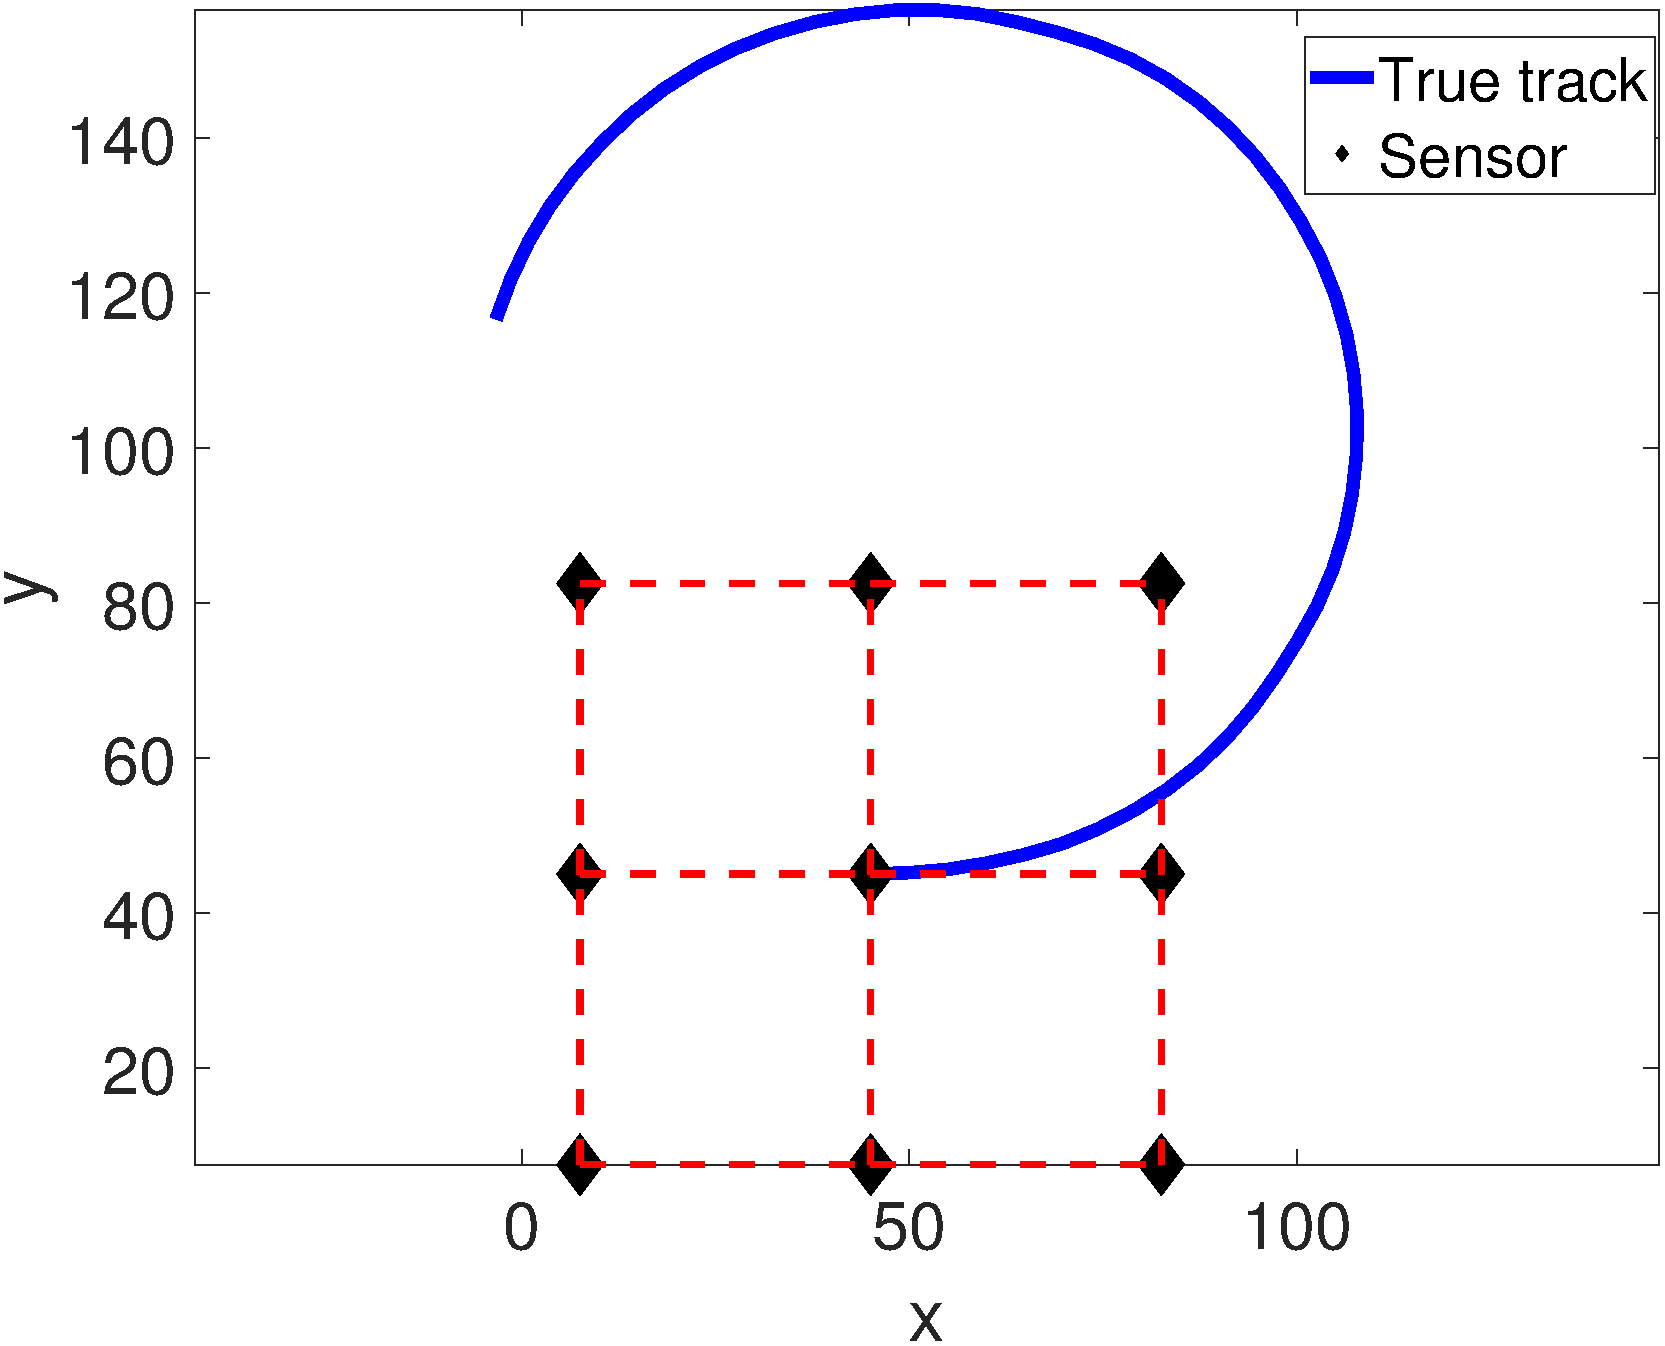
\includegraphics[width=0.75\textwidth]{Figures/track}
\caption{Target trajectory (blue curve) and sensor positions (red diamond)}
\label{fig:track}
\end{figure}

\subsection{Algorithm setup}
All particle filters use a total of $N=1000$ particles. At time step 1, we generate the initial particles using the true target state: $X_i(1) \sim \mathcal{N}(X(1), R_{\text{initial}})$ with $R_{\text{initial}}=\text{diag}([0.5^2,0.5^2,0.05^2,0.05^2])$. 

For LCpf, we use a set of basis functions involving all permutations of $x_t^iy_t^j$ with $0\leq i, j \leq d$ where $d$ is some user-specified max degree. For $d=2$, the basis functions would be
\begin{align*}
\beta_1(X) &= x_t^0 y_t^0 = 1 \\
\beta_2(X) &= x_t^0 y_t^1 = y_t \\
\beta_3(X) &= x_t^0 y_t^2 = y_t^2 \\
\beta_4(X) &= x_t^1 y_t^0 = x_t \\
... \\
\beta_9(X) &= x_t^2 y_t^2 
\end{align*}

For LApf, we construct a $K$-nearest neighbor graph and retain $m< N$ Eigenvectors as the basis of Laplacian transformation. 

For Clusterpf, all particles are grouped into $C$ clusters and a $K$-nearest neighbor graph is constructed to recover individual particle weights. 

Finally, the random number generators are synchronized to ensure that the particles remain the same across sensors. All summations are computed exactly without using any distributed algorithms. This ensures that no performance degradation is caused by consensus.

\subsection{Individual algorithm performance}
In this section, we evaluate the performance of individual algorithms with respect to their specific parameters. We run a number of Monte Carlo simulations on each algorithm while varying one single parameter. The track remains the same in each trial; but the measurements differ. 

We evaluate the algorithms' performances using two criterion: \textit{root mean squared error} (RMSE) of position estimate and total runtime (from initialization to end of time step 50). Our objective is to select a set of parameters that offer optimal trade-off between tracking performance and computational load. 

Consider first LCpf. The max degree $d$ should offer a trade-off between tracking performance and total runtime. Higher degree $d$ leads to more basis functions and likely better approximation of the measurement model. On the other hand, more basis functions lead to more computation and longer runtime. 

\begin{figure}
\centering
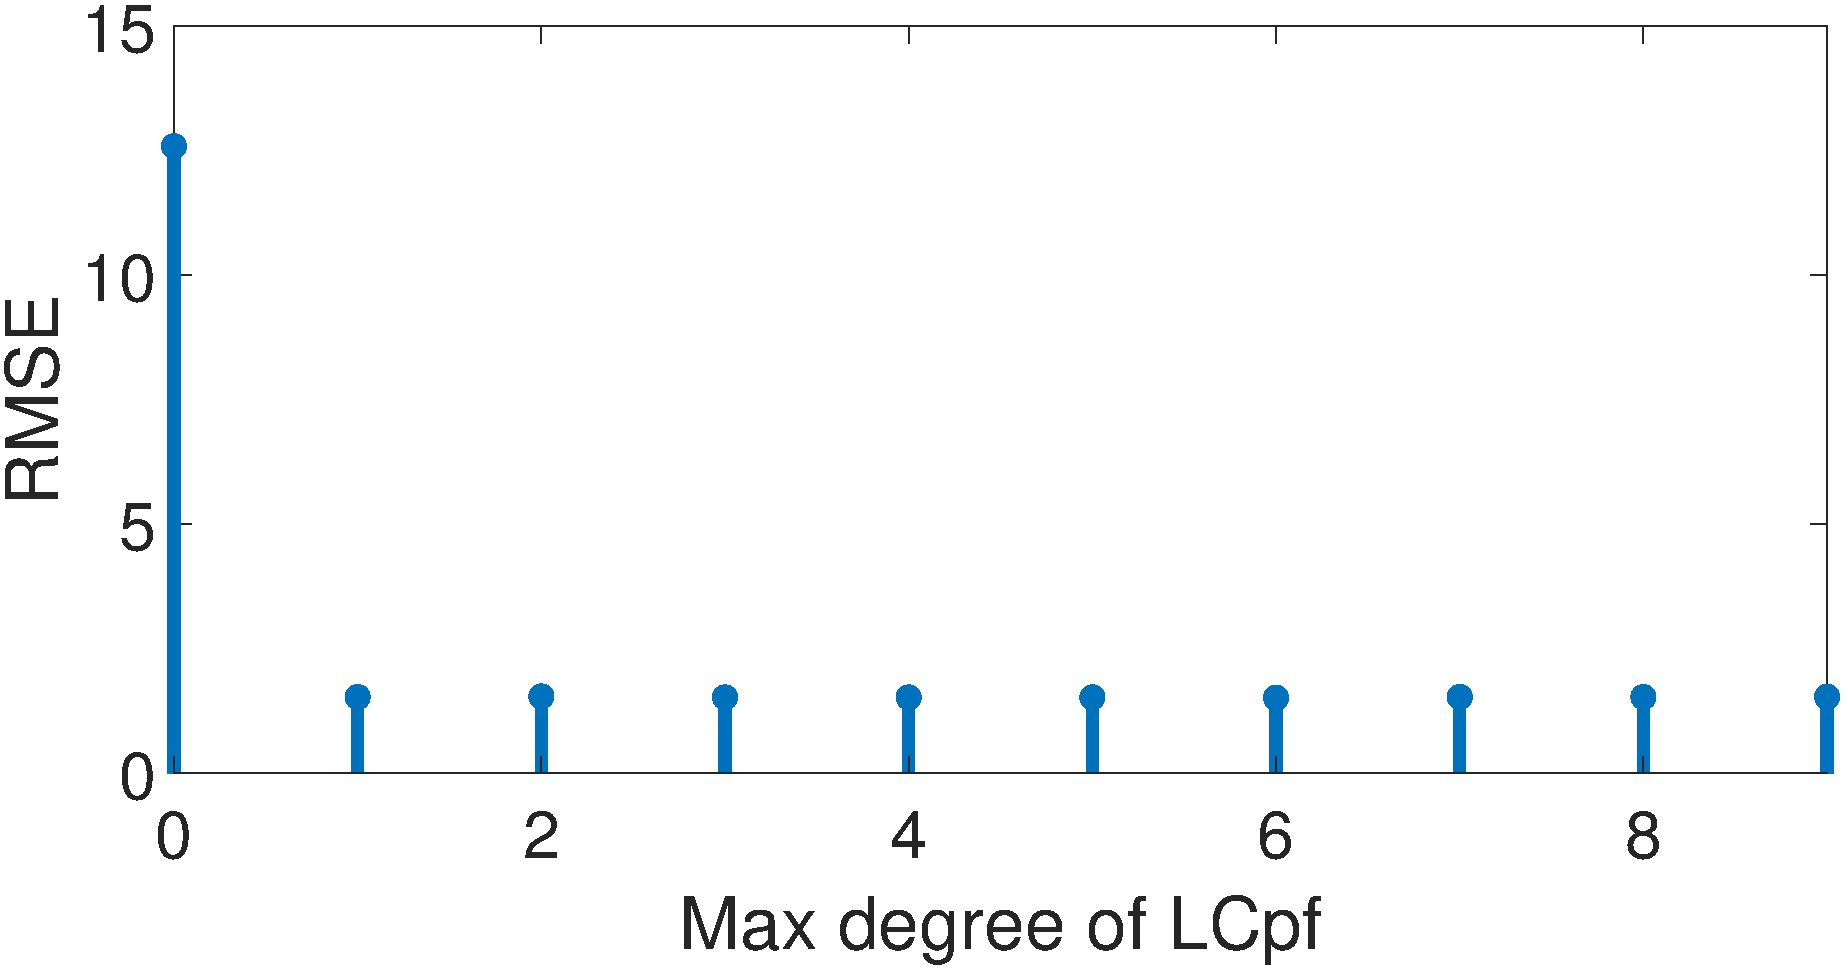
\includegraphics[width=0.45\textwidth]{Figures/RMSE_maxDegree}
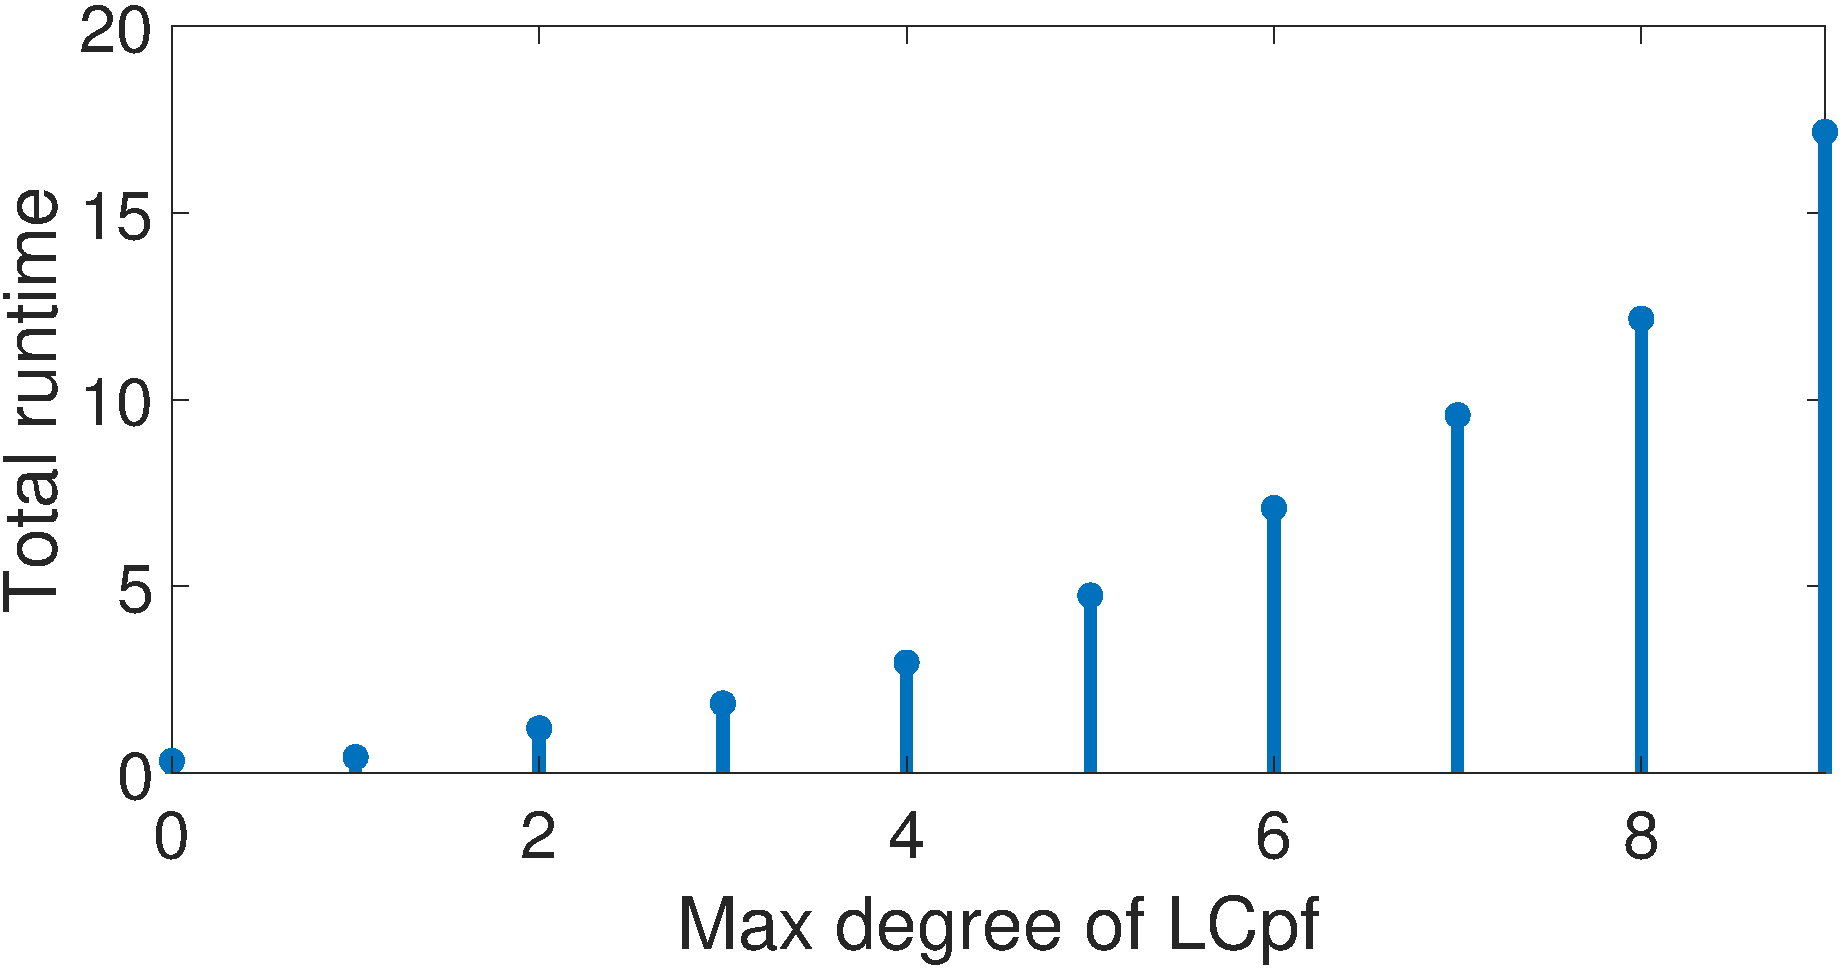
\includegraphics[width=0.45\textwidth]{Figures/runtime_maxDegree}
\caption{Boxplot of RMSE and runtime of LCpf with respect to max degree for 200 Monte Carlo trials}
\label{fig:results_maxDegree}
\end{figure}

Fig.~\ref{fig:results_maxDegree} shows the boxplot of time-averaged RMSE and total runtime over 200 Monte Carlo trials. The total runtime increases with larger max degree as expected. On the other hand, we do not see any significant difference in RMSE for $1\leq d \leq 9$. This suggests that the additional basis functions for $d>1$ do not yield a better approximation of the measurement model. Therefore, we will select $d=1$ for LCpf in subsequent simulations. 

Consider next LApf. This filter has two parameters of interest: $K$, the number of nearest neighbors for the particle graph, and $m$, the number of Eigenvectors for the transformation. Different values of $K$ yield different graphs over the same particles and by extension different Eigenvectors. Retaining more Eigenvectors yields a better approximation of particle log-likelihoods at the cost of higher computation overhead. 

Fig.~\ref{fig:RMSE_NbEigen} shows the boxplot of time-averaged RMSE over 100 trials. For all values of $K$, we do not notice a significant improvement in tracking performance as more Eigenvectors are used. This suggests that most of the graph energy is stored in the first 50 Eigenvectors

Fig.~\ref{fig:runtime_NbEigen} shows the boxplot of total runtime. There is a lot of fluctuations in the runtime; but we do notice an overall decrease as we increase $m$. This result is rather surprising to us and we are still looking into the cause of this behavior. For the subsequent simulations, we will set $K=5$ and $m=500$. 

\begin{figure}
\centering
\subfigure[$K$=5]{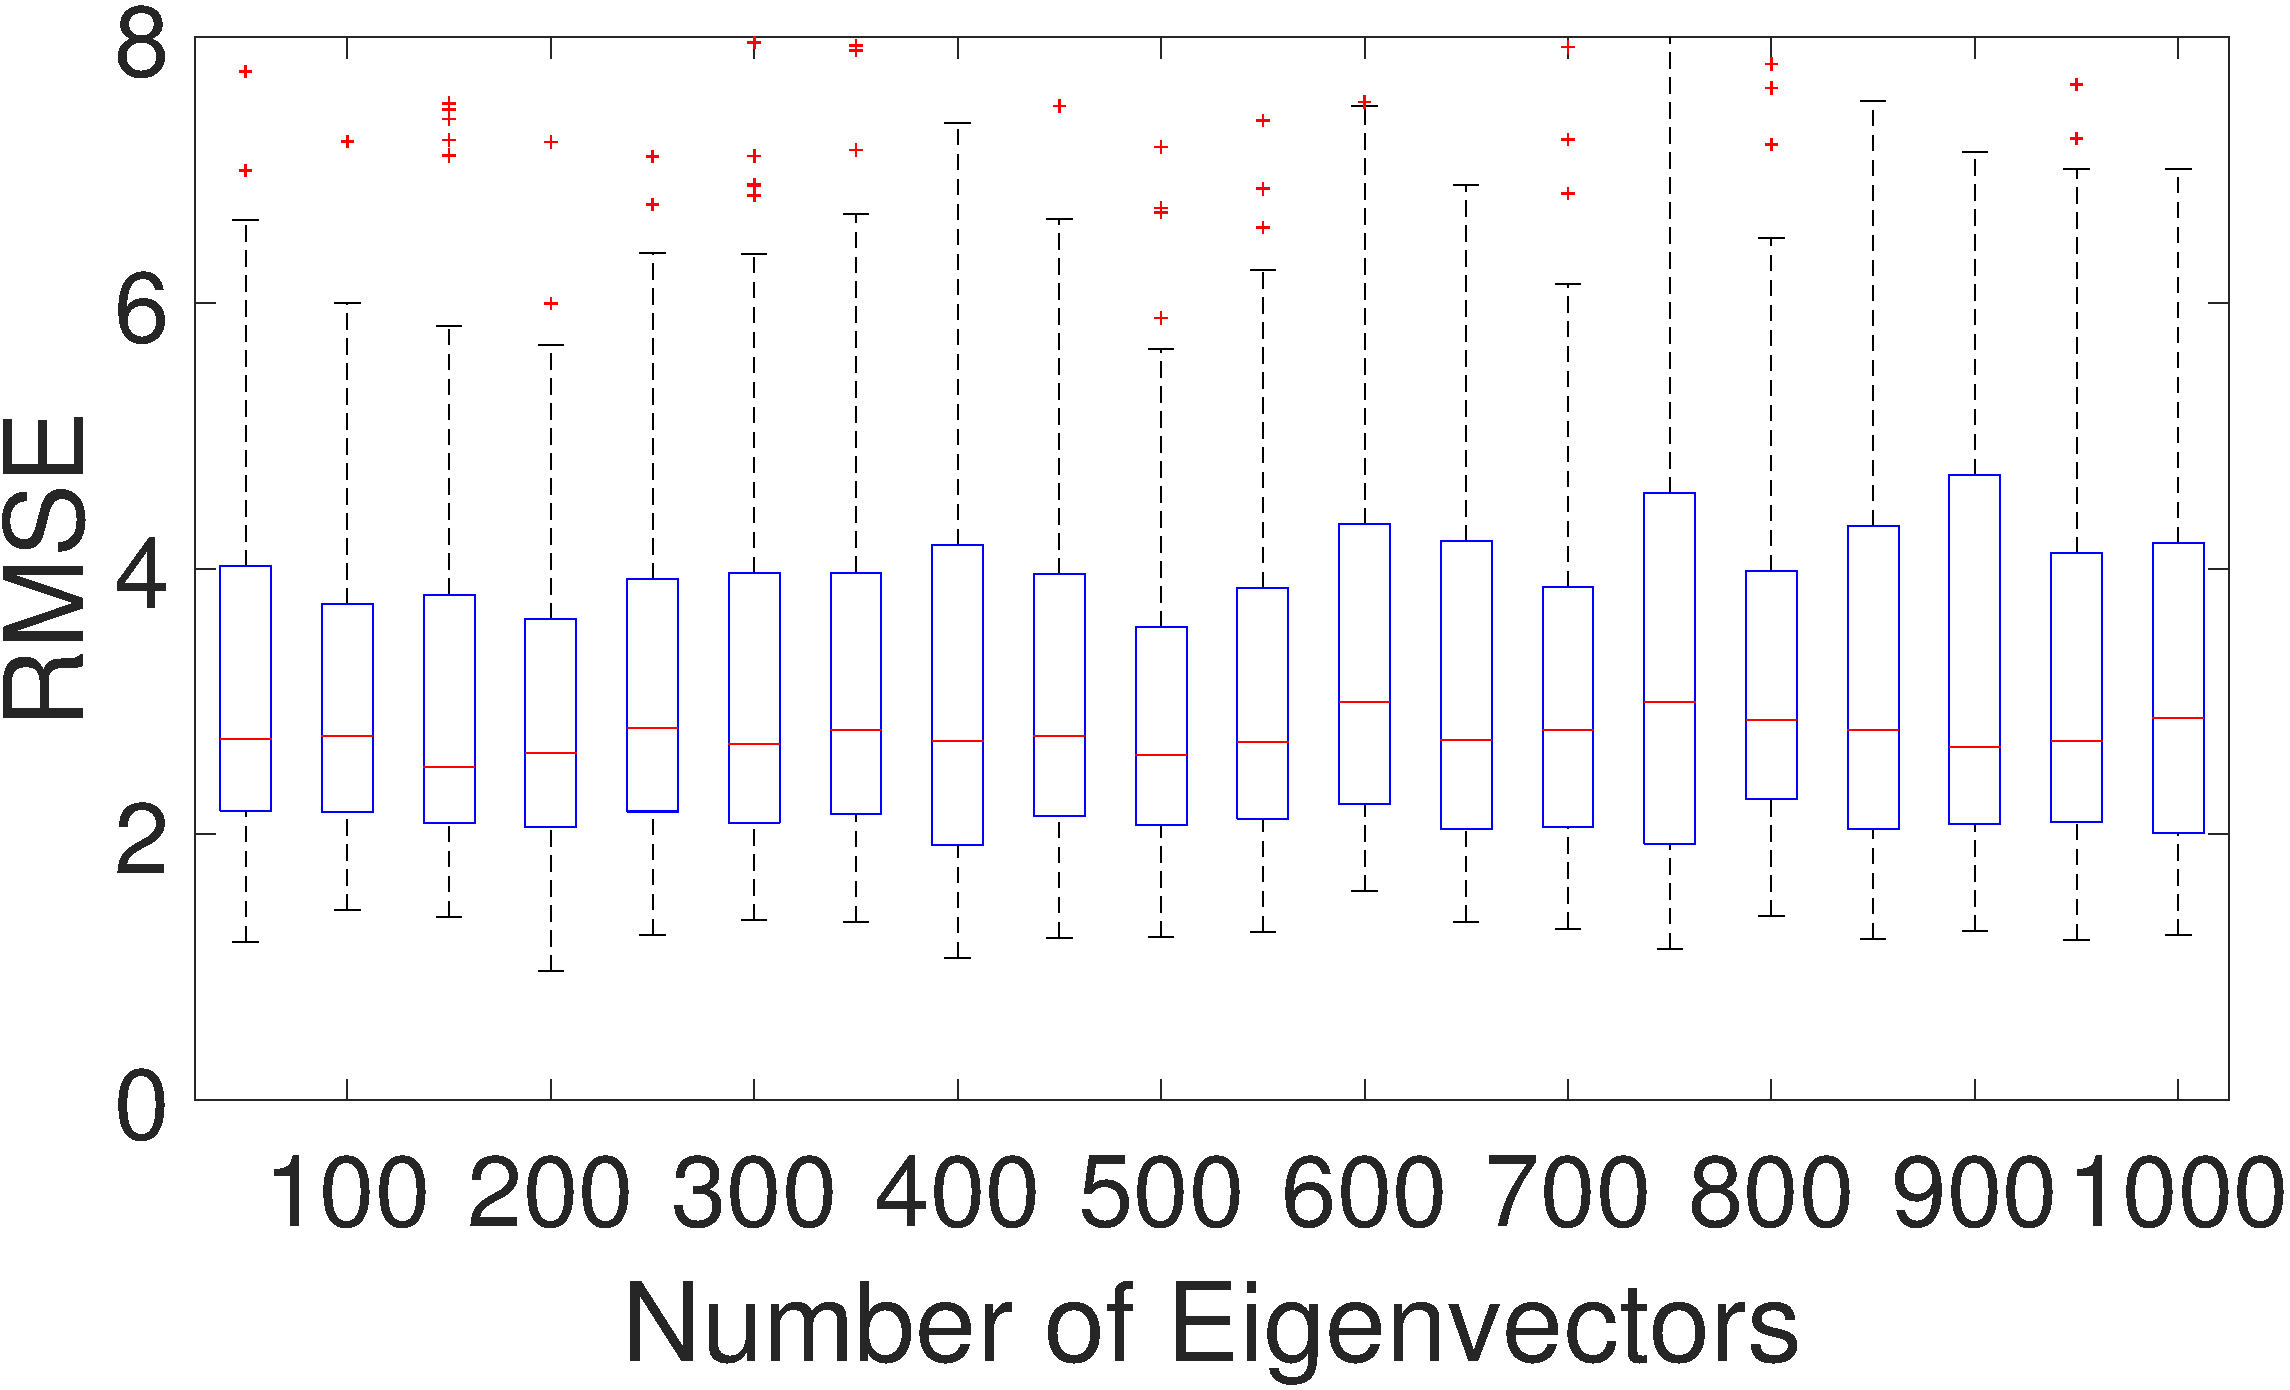
\includegraphics[width=0.3\textwidth]{Figures/RMSE_NbEigen_KNN5}}
\subfigure[$K$=10]{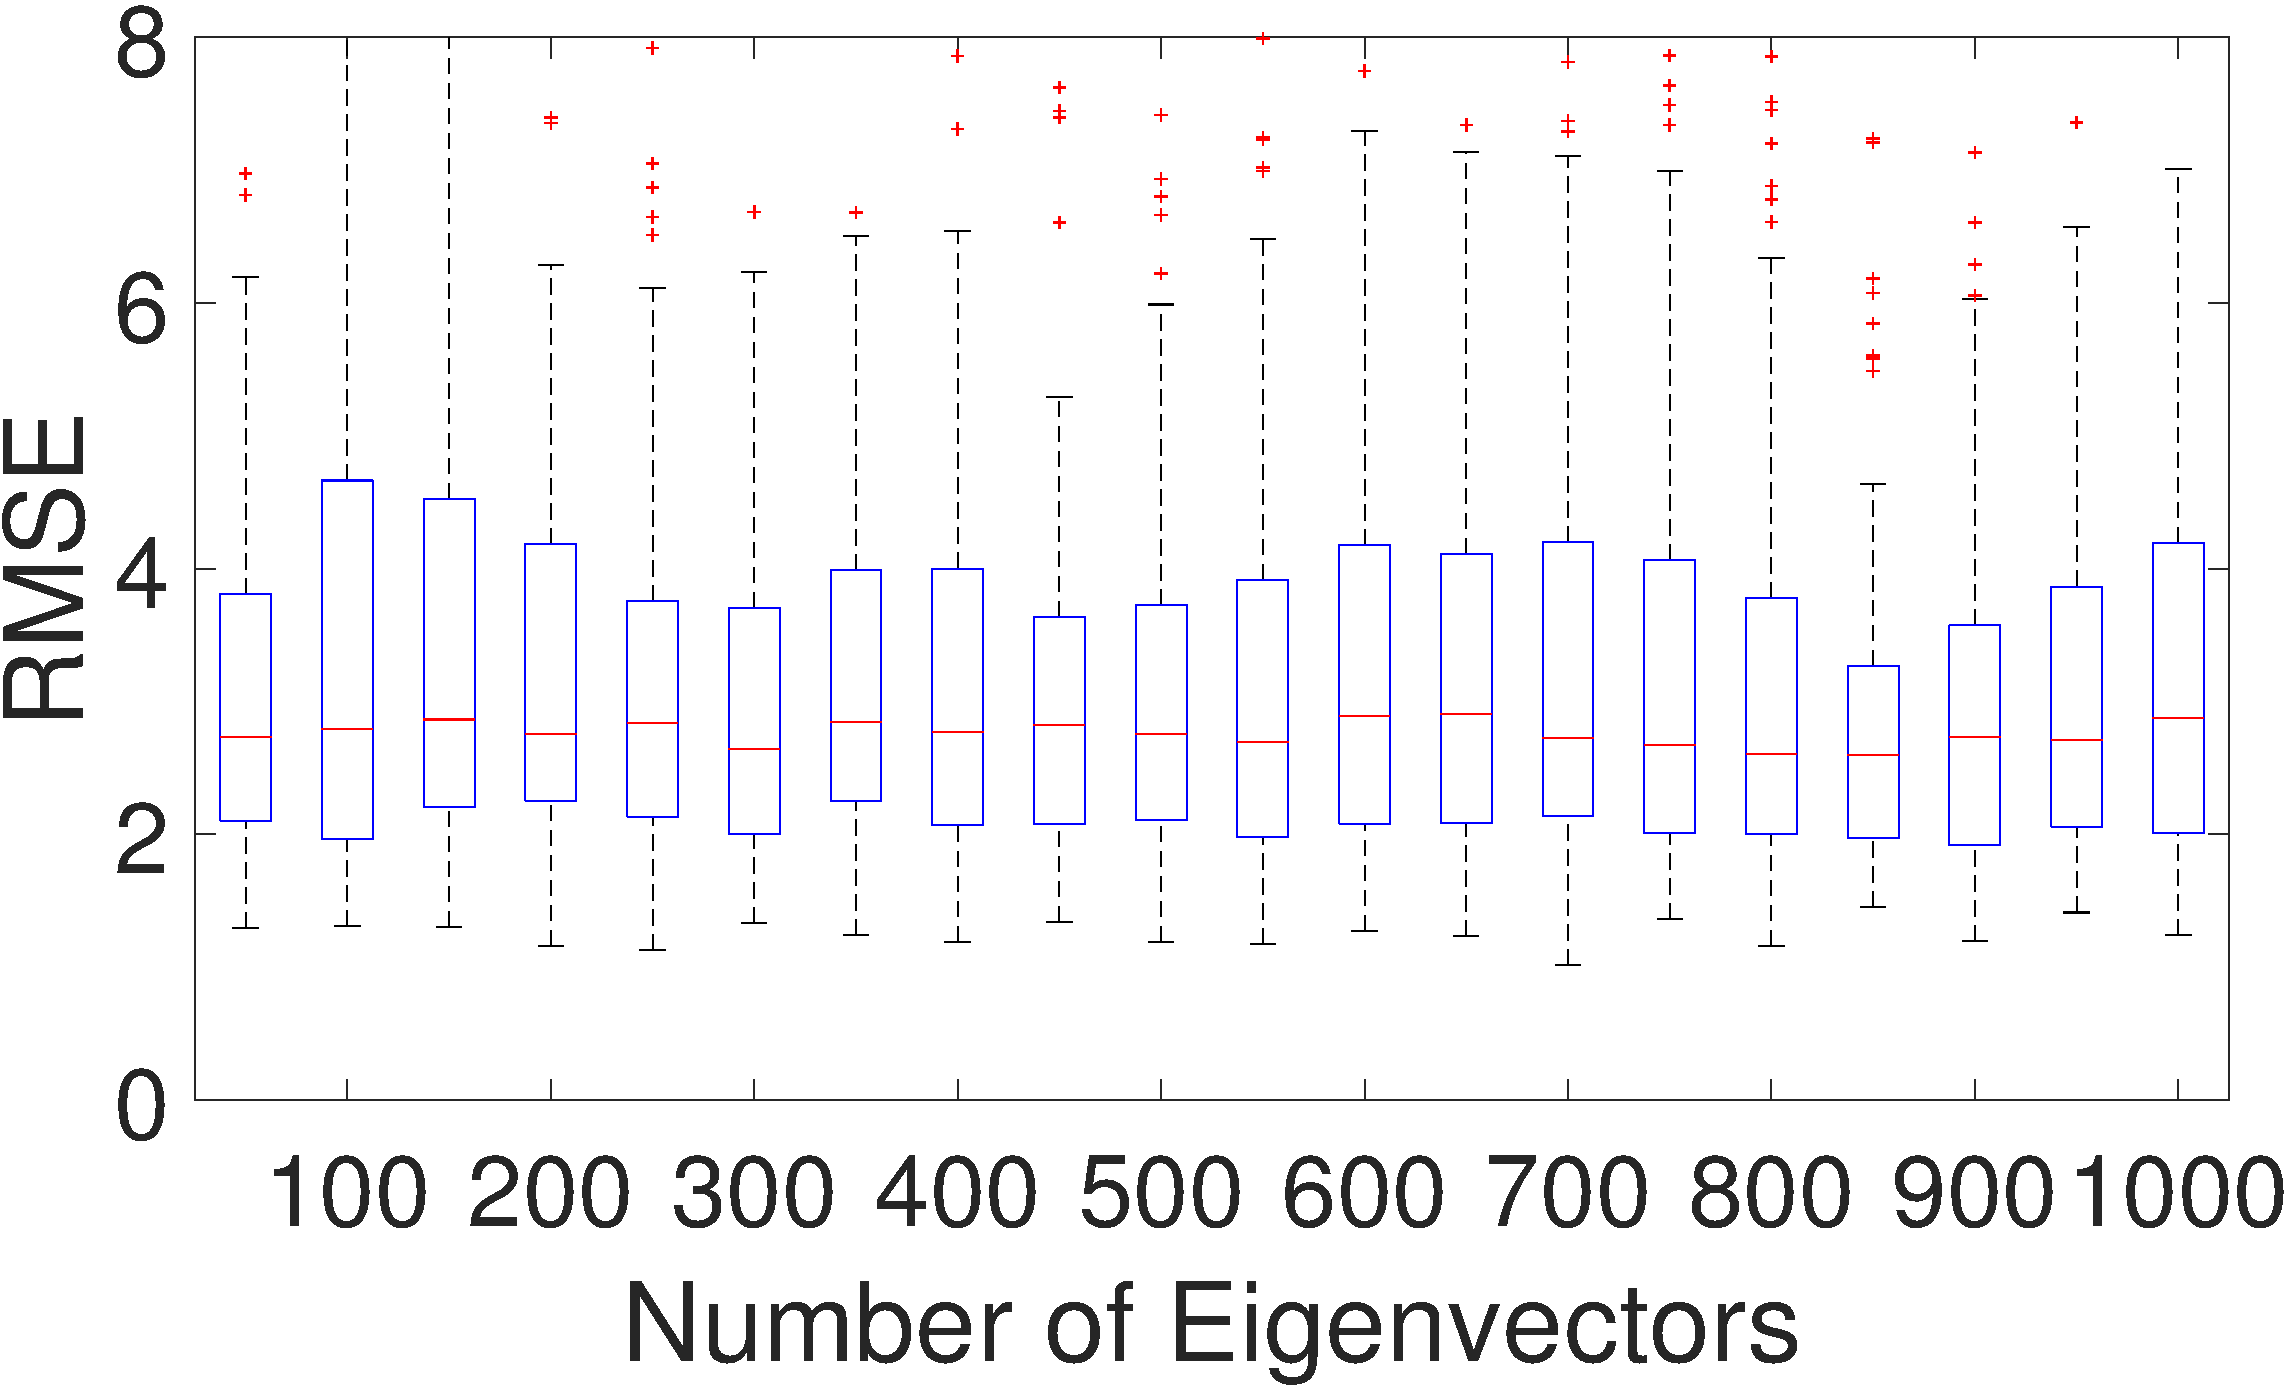
\includegraphics[width=0.3\textwidth]{Figures/RMSE_NbEigen_KNN10}}
\subfigure[$K$=20]{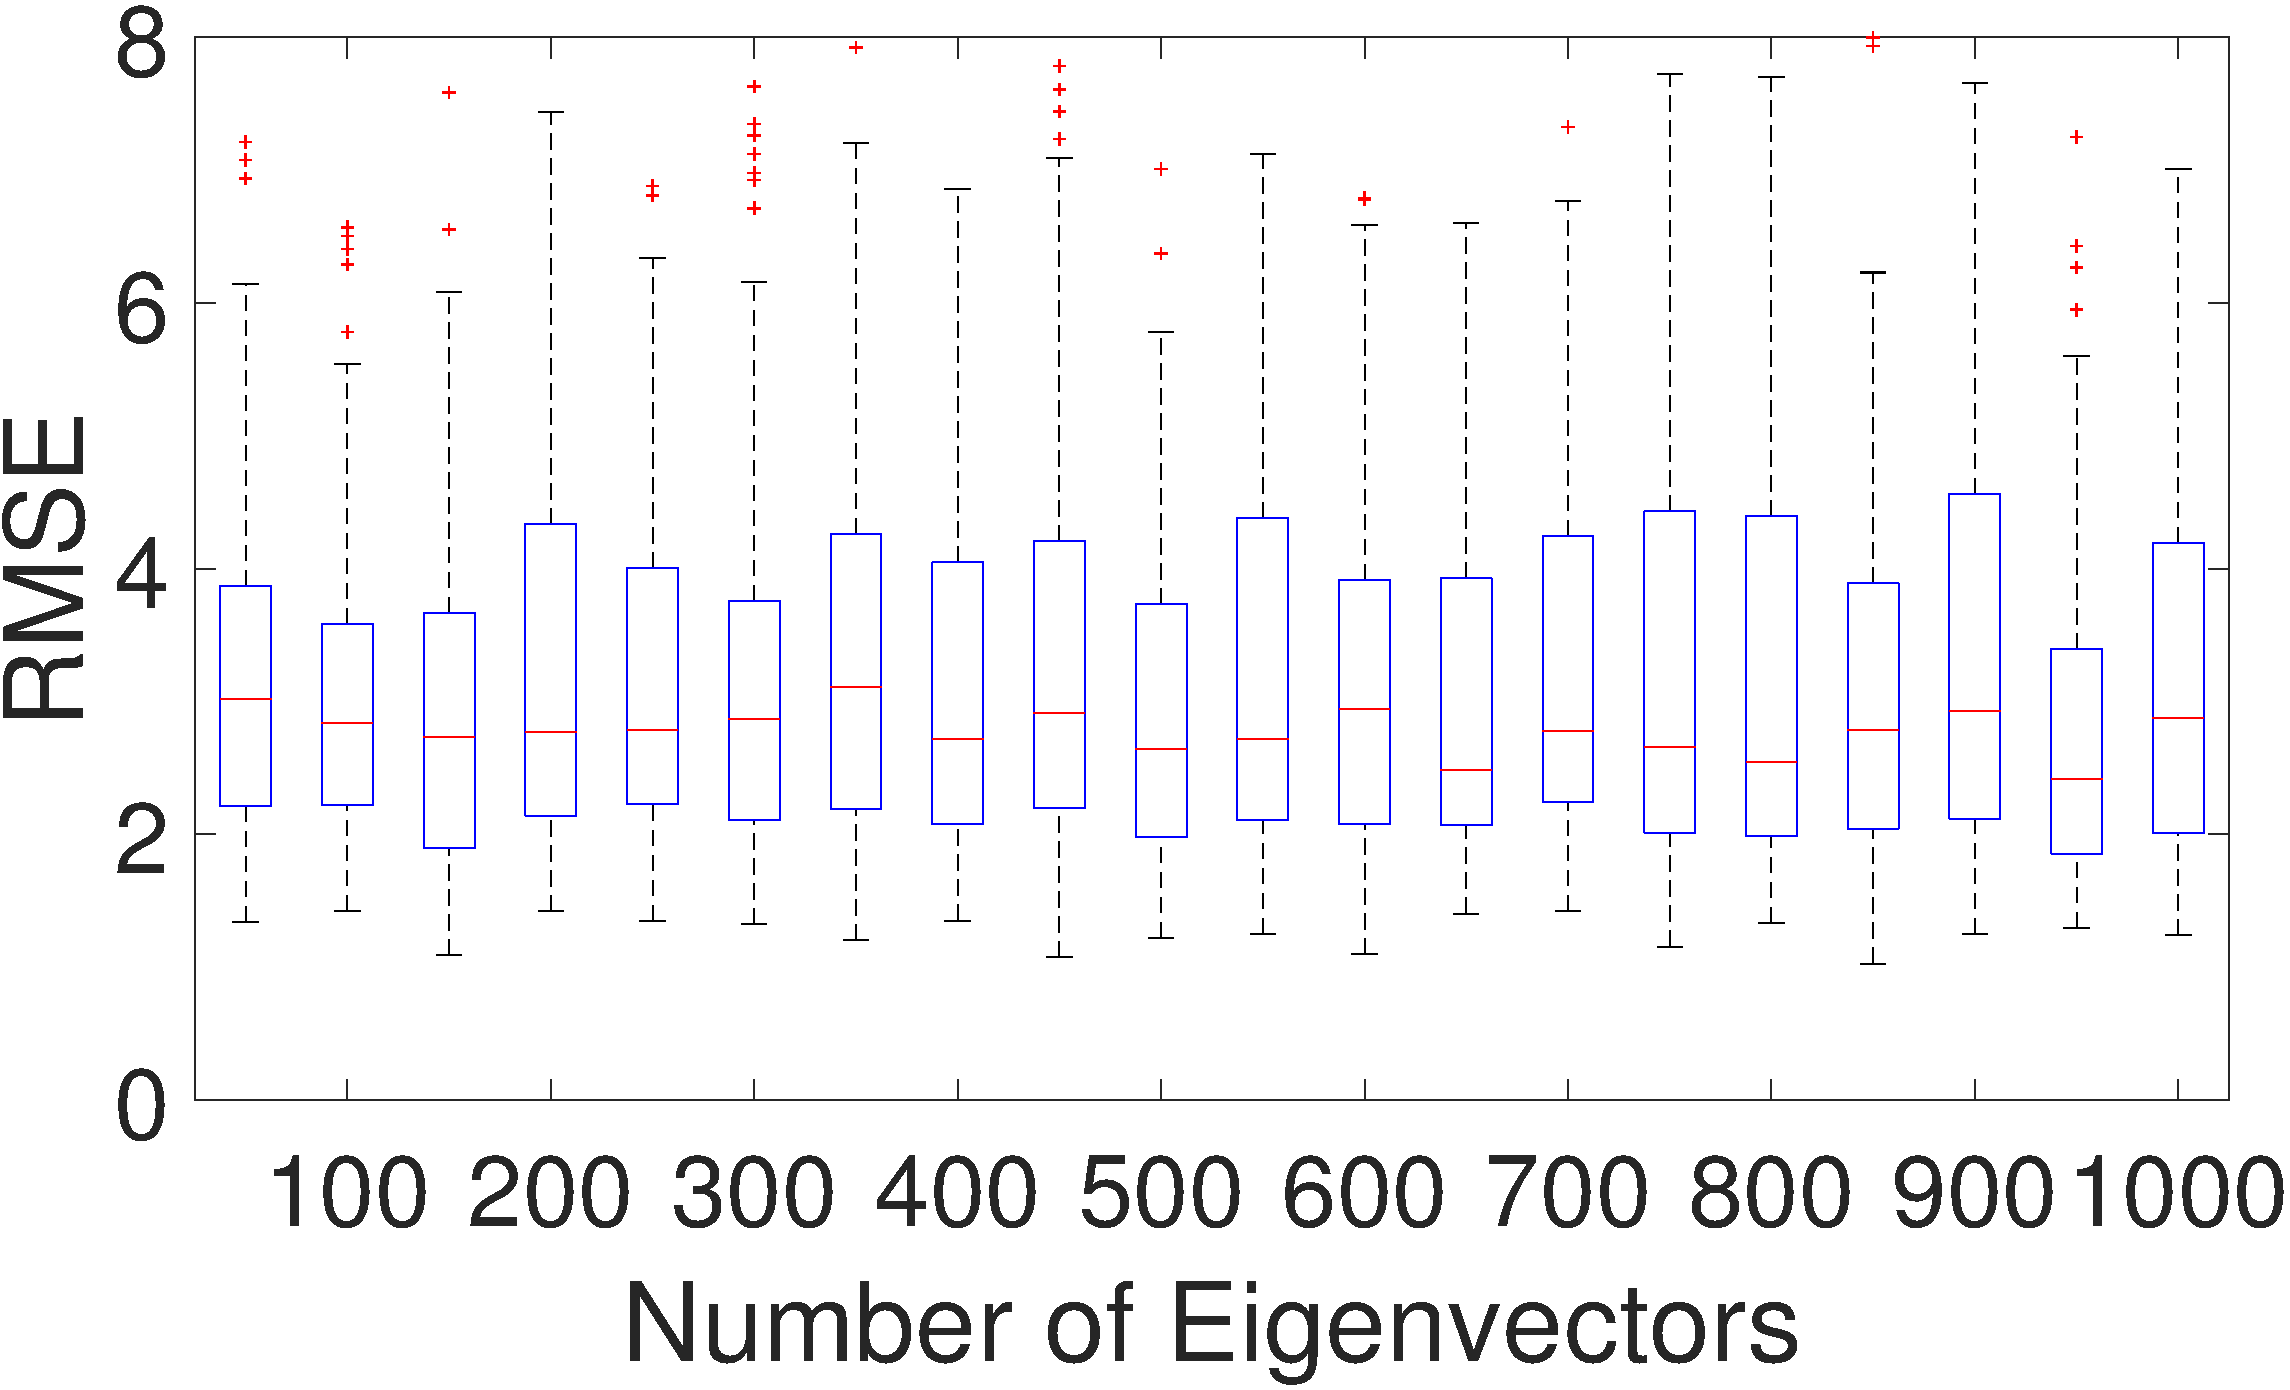
\includegraphics[width=0.3\textwidth]{Figures/RMSE_NbEigen_KNN20}}
\caption{Boxplot of time-averaged RMSE of LApf with respect to the number of eigenvectors over 100 Monte Carlo trials for different values of $K$.}
\label{fig:RMSE_NbEigen}
\end{figure}

\begin{figure}
\centering
\subfigure[$K$=5]{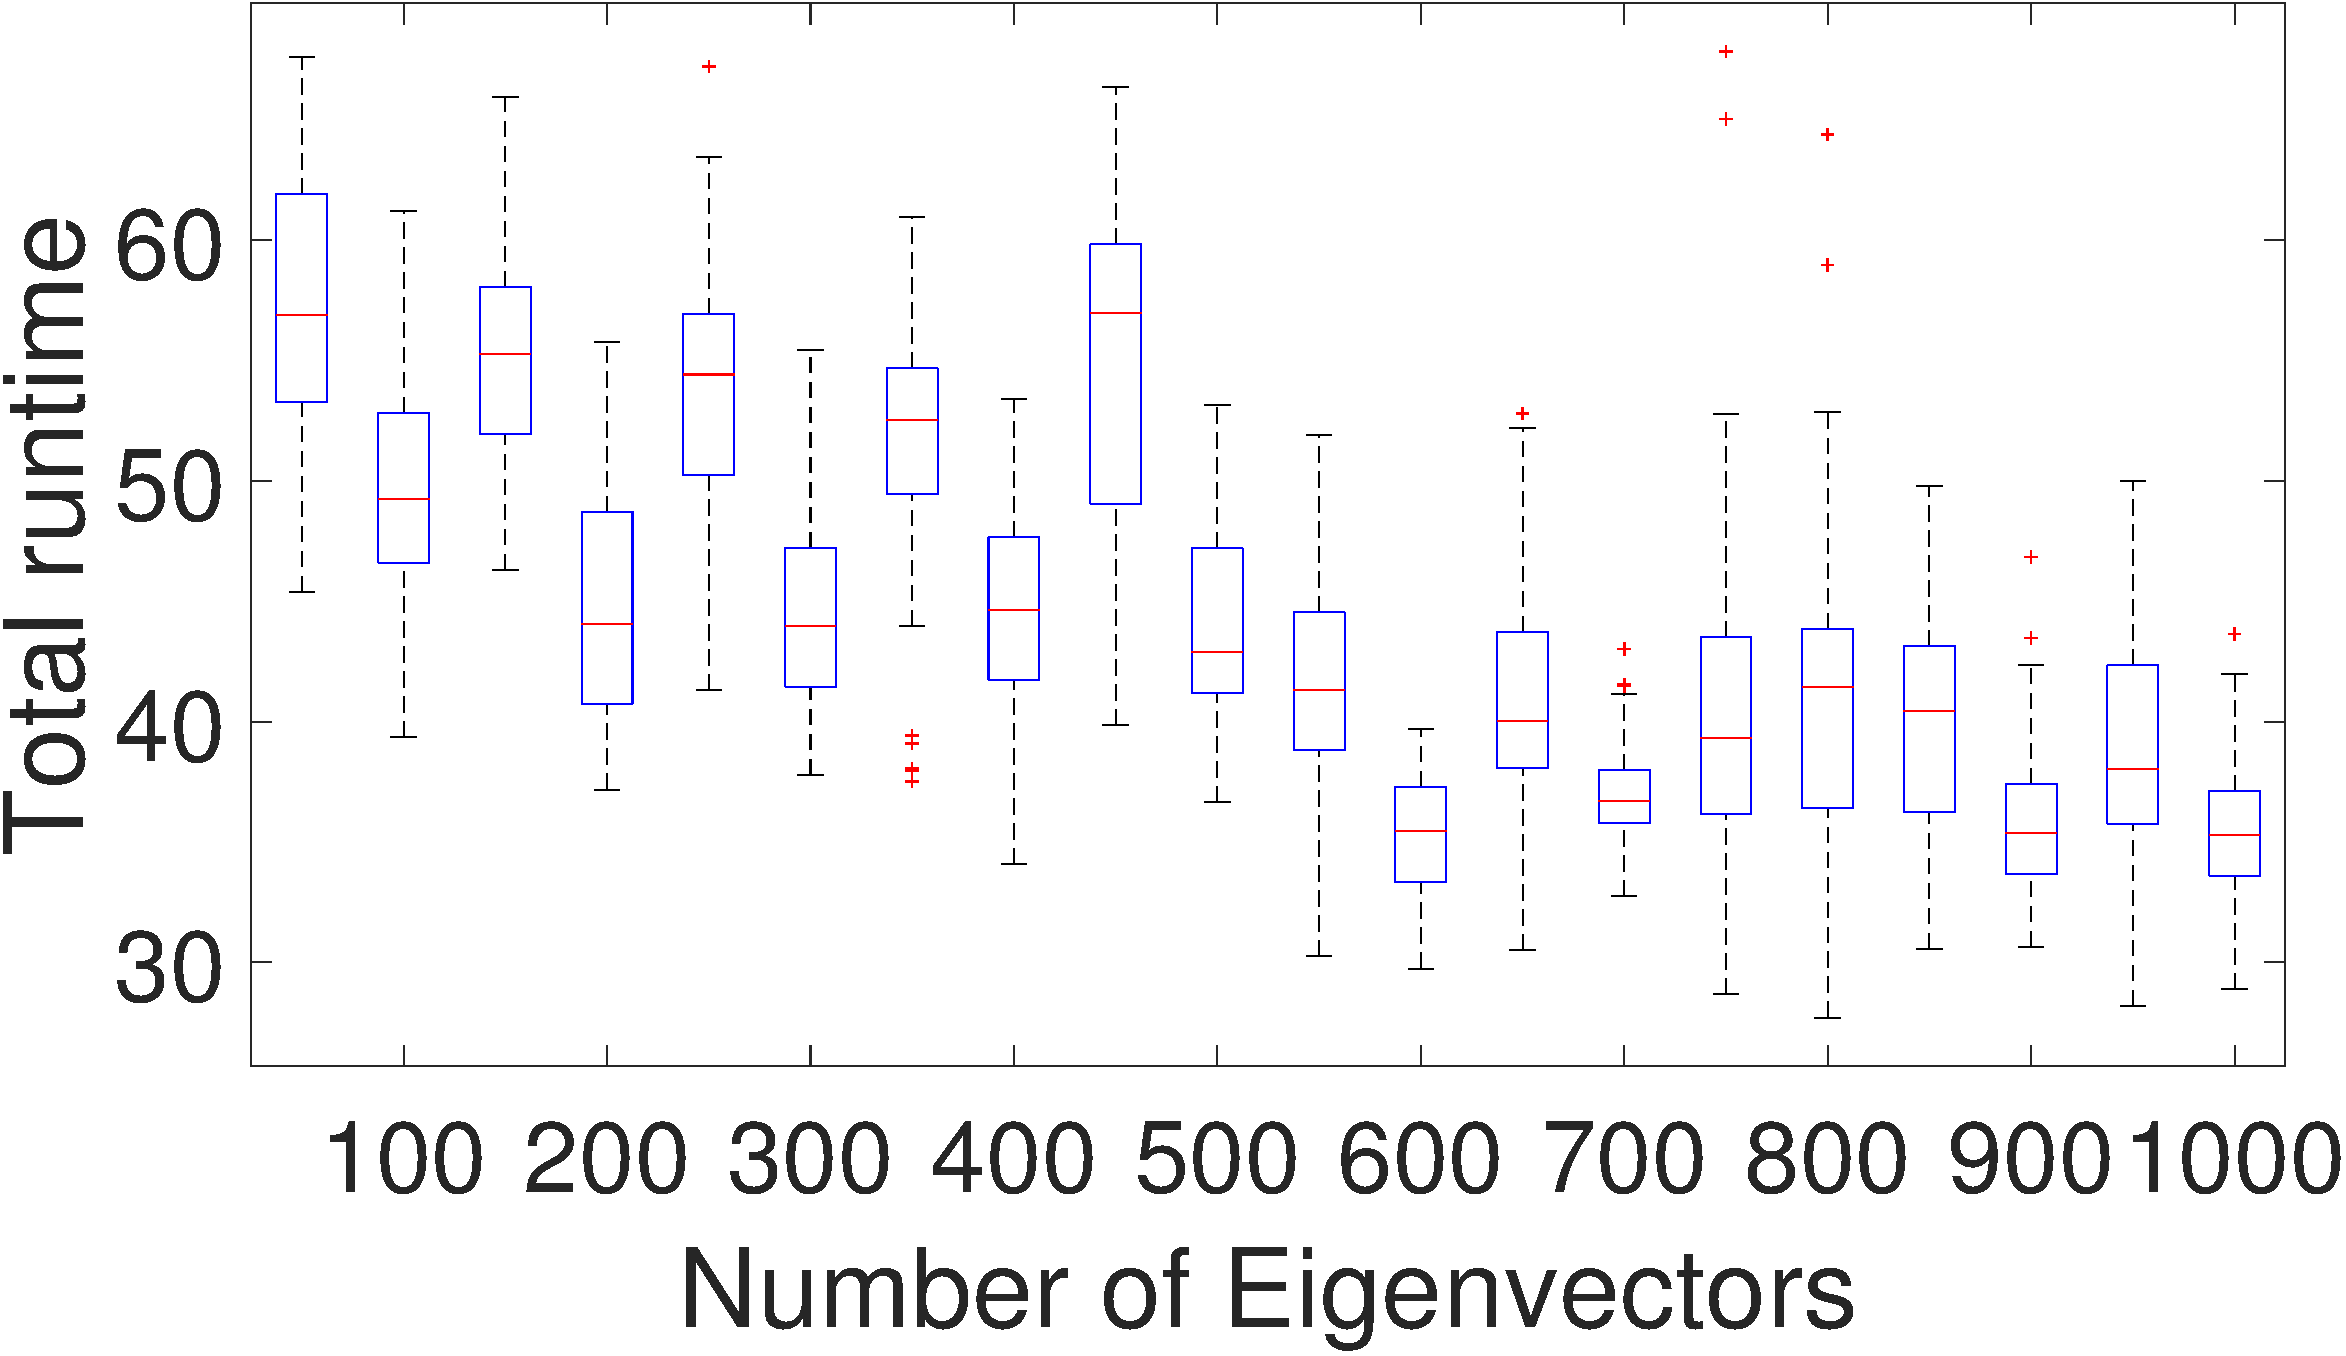
\includegraphics[width=0.3\textwidth]{Figures/runtime_NbEigen_KNN5}}
\subfigure[$K$=10]{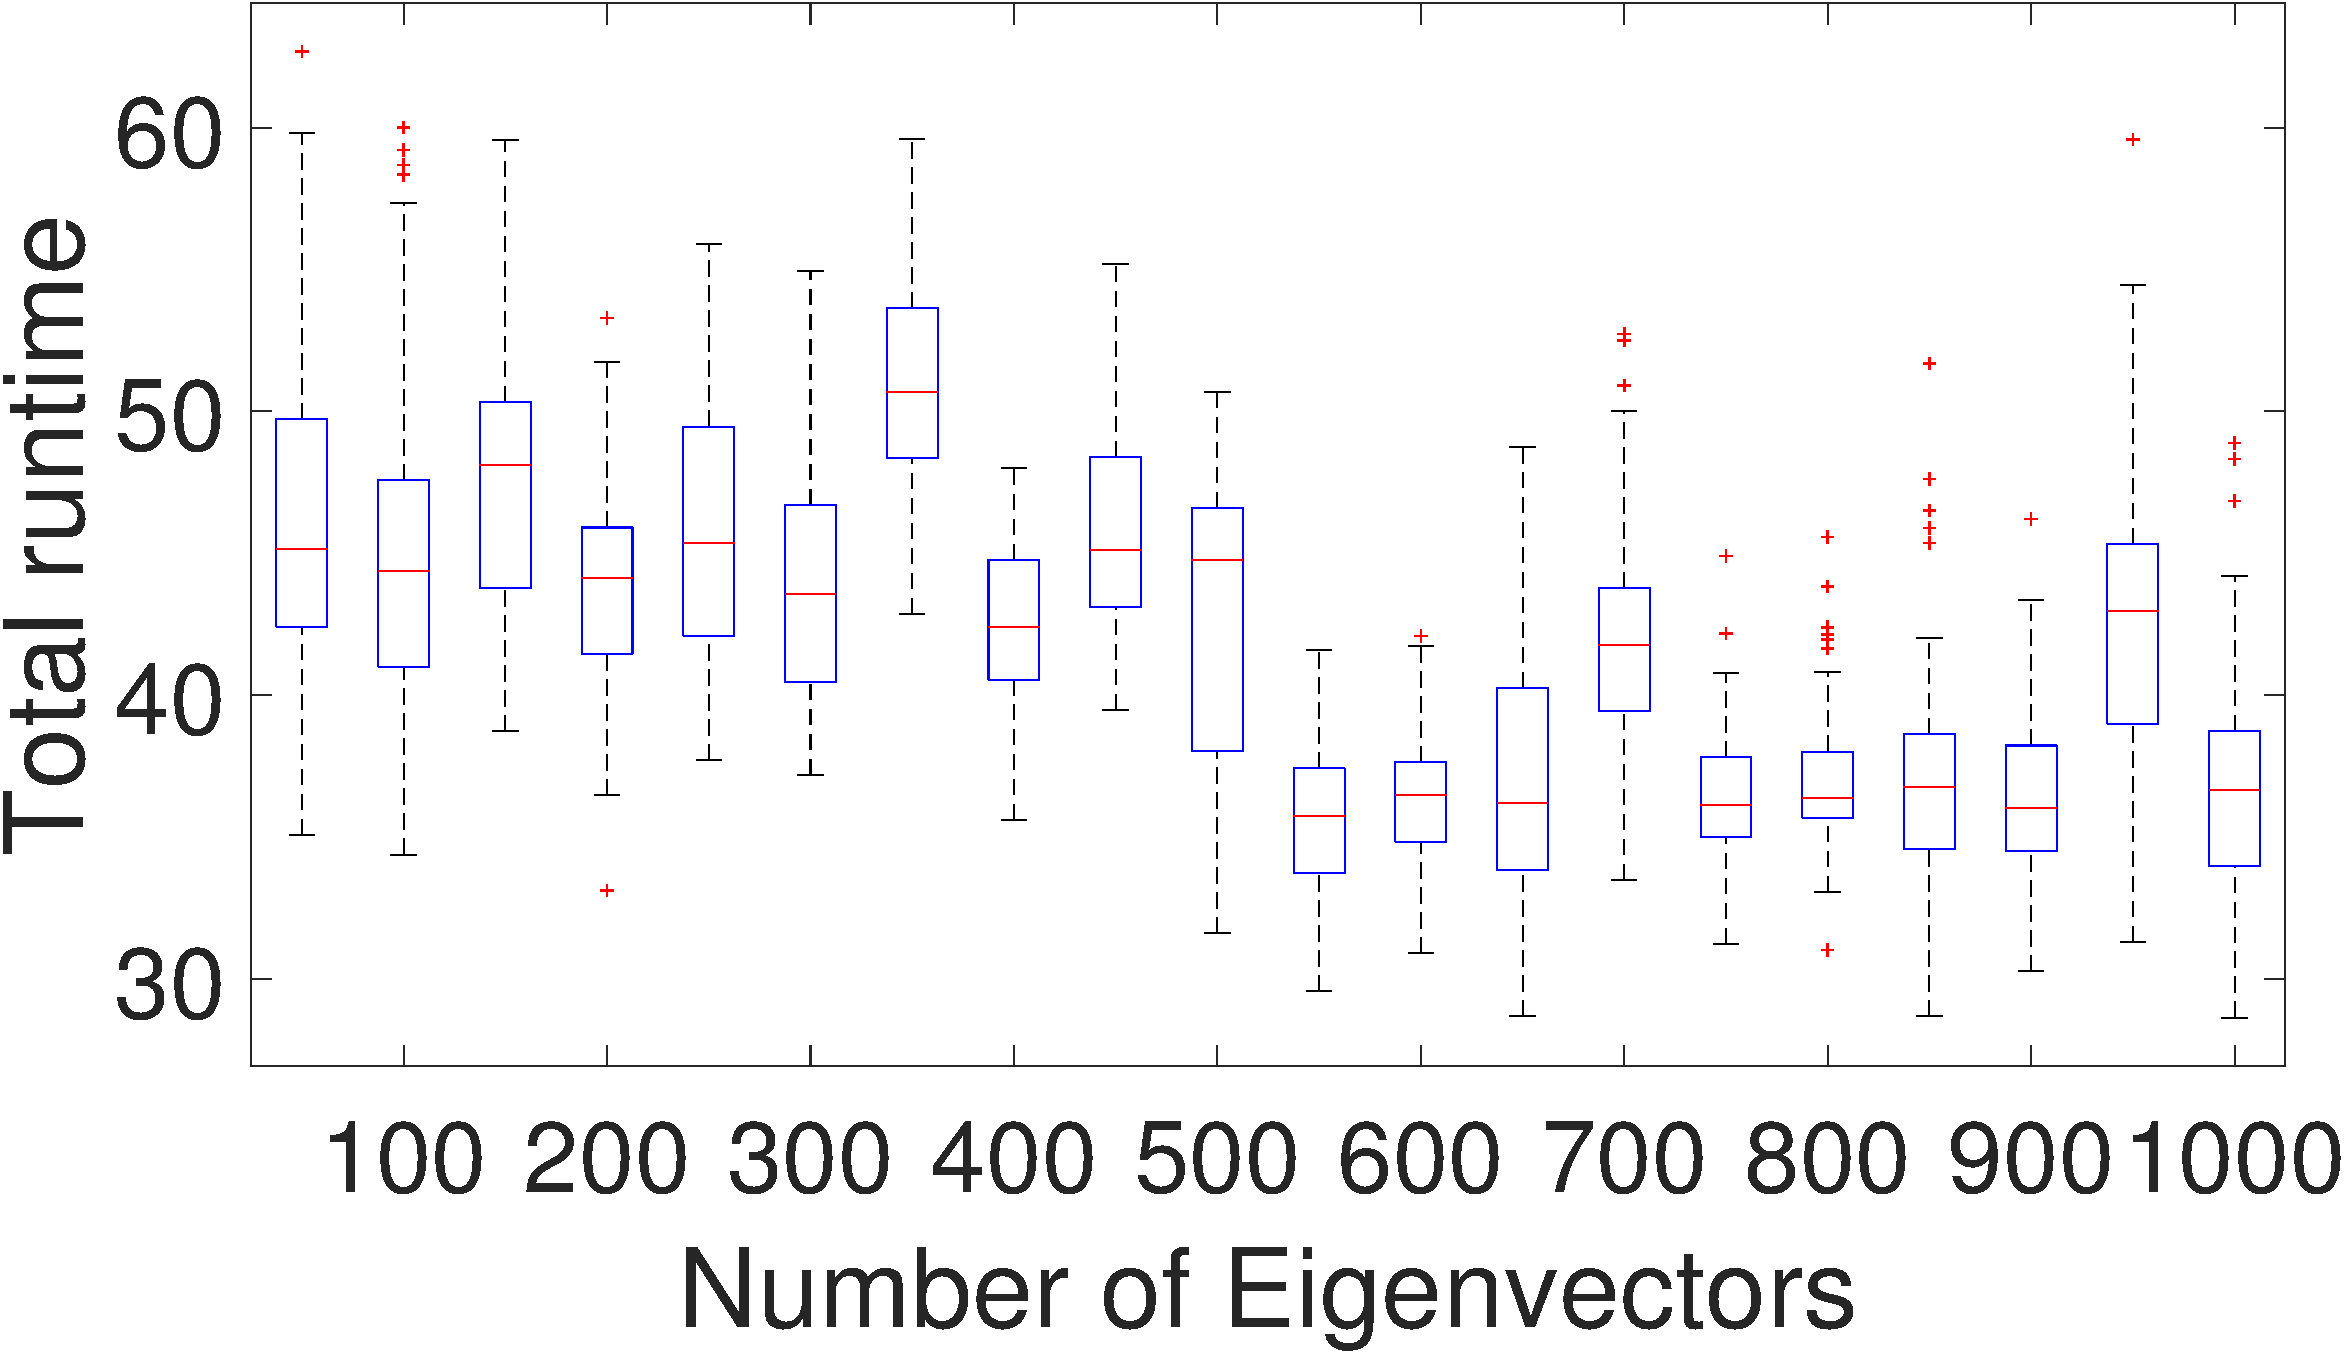
\includegraphics[width=0.3\textwidth]{Figures/runtime_NbEigen_KNN10}}
\subfigure[$K$=20]{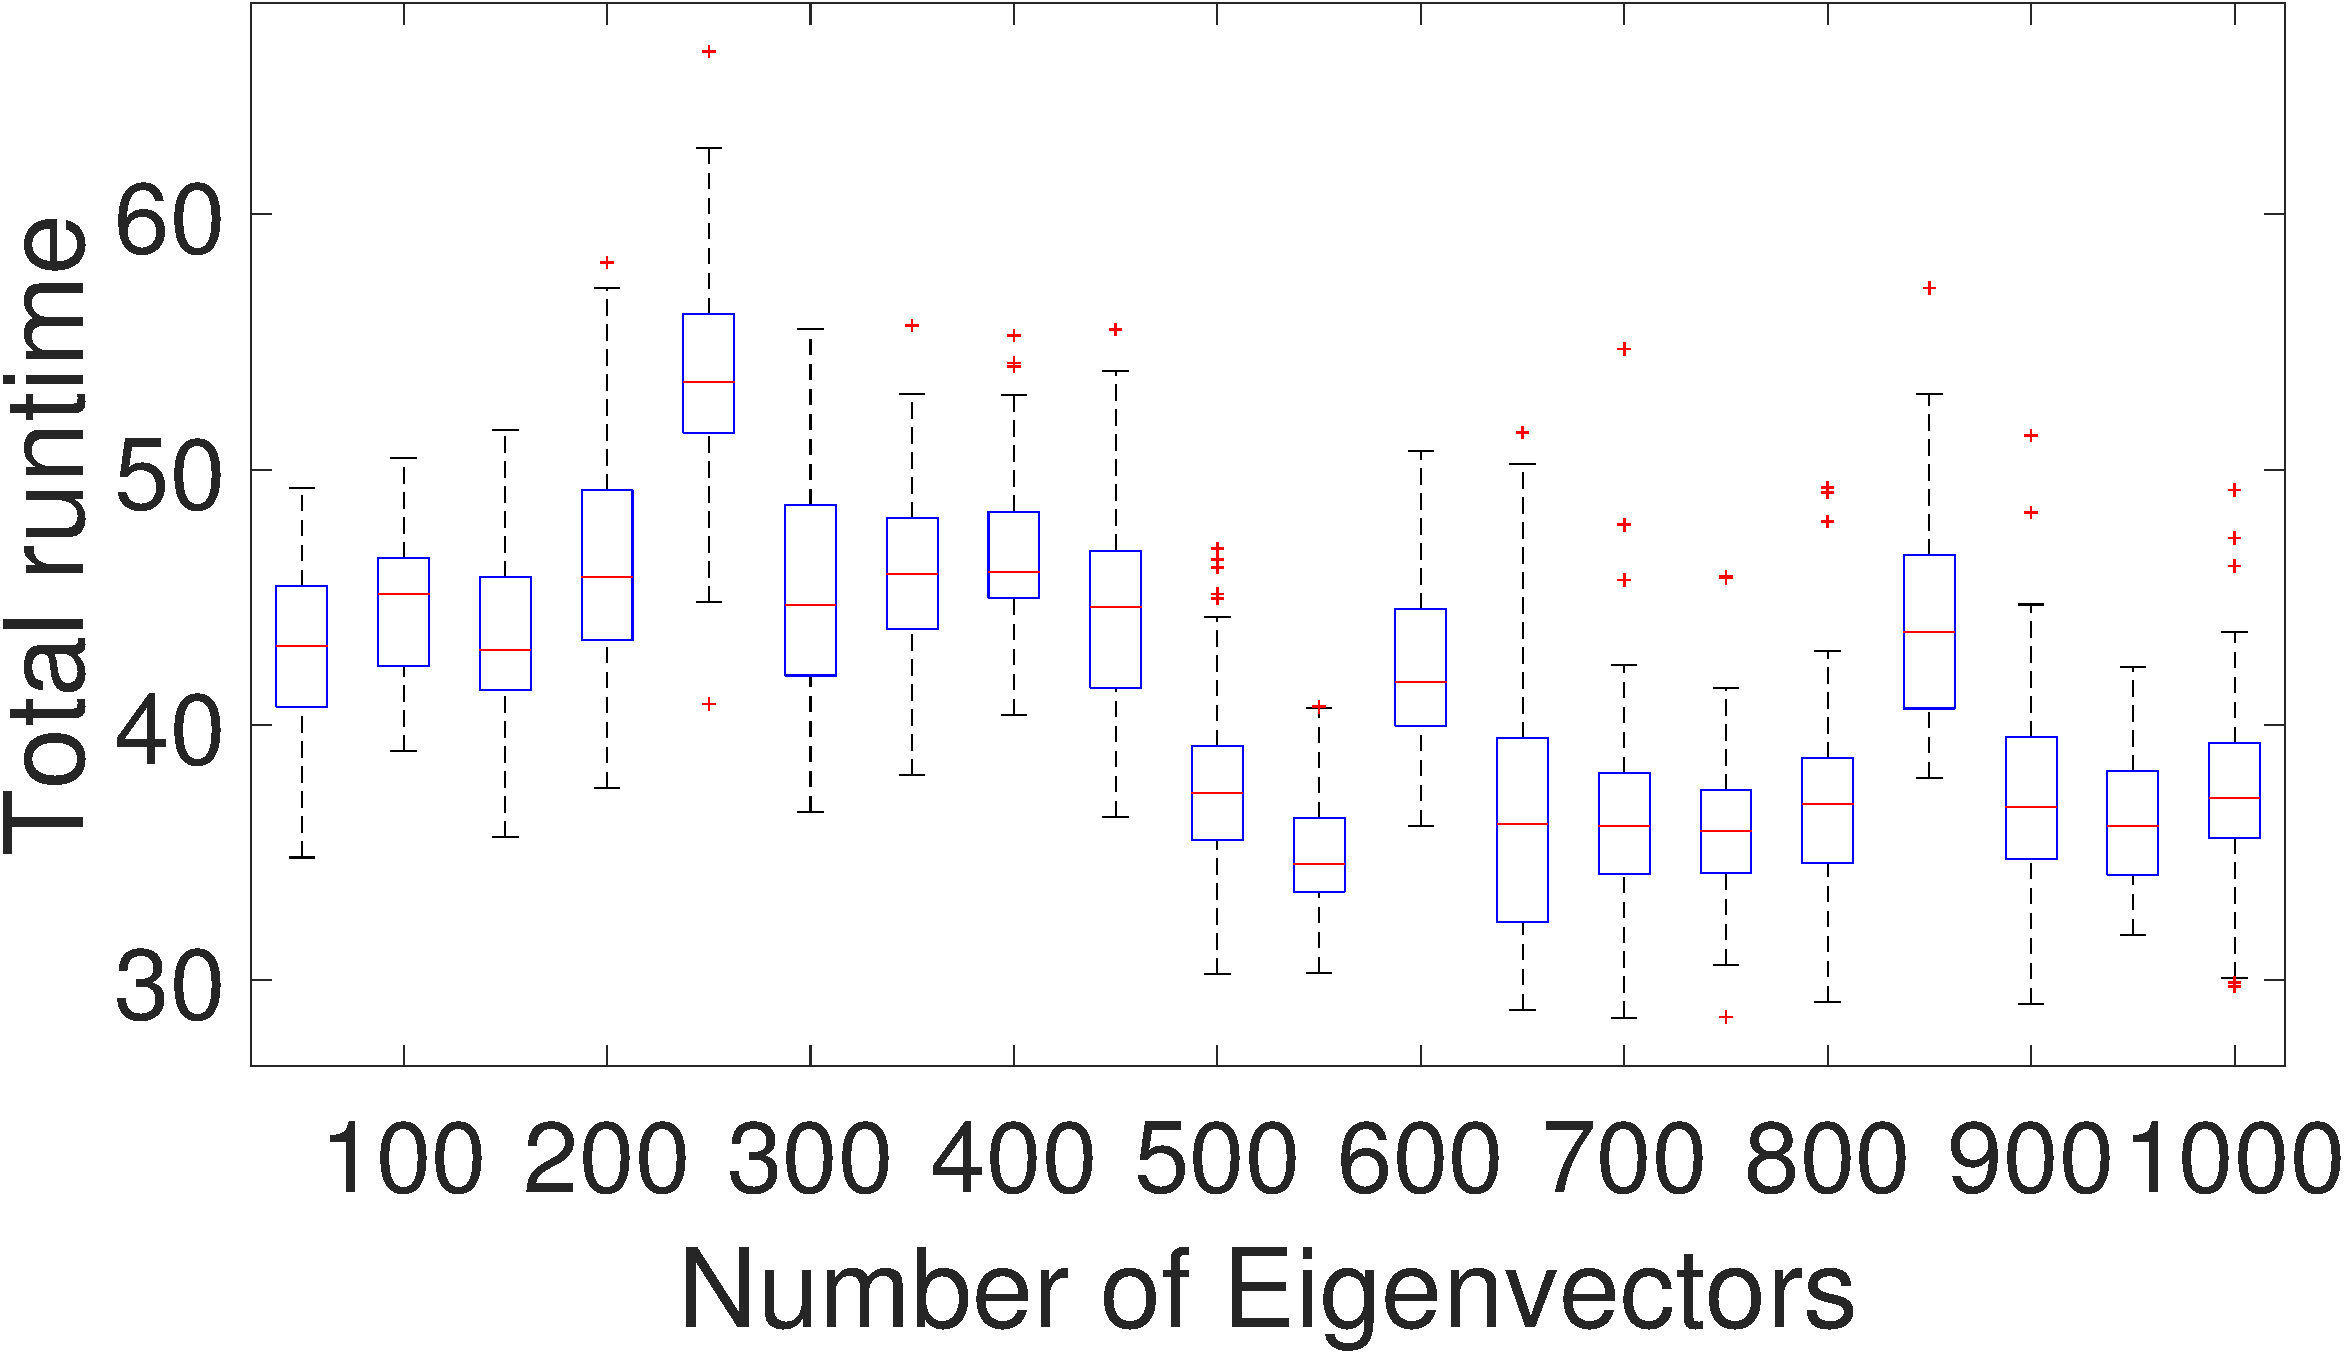
\includegraphics[width=0.3\textwidth]{Figures/runtime_NbEigen_KNN20}}
\caption{Boxplot of total runtime of LApf with respect to the number of eigenvectors over 100 Monte Carlo trials for different values of $K$.}
\label{fig:runtime_NbEigen}
\end{figure}

Finally, consider Clusterpf. This filter also has two parameters of interest: number of clusters $C$ and number of neighbors $K$ for the graph construction. Fig.~\ref{fig:RMSE_NbClusters} and Fig.~\ref{fig:runtime_NbClusters} show the boxplots of time-averaged RMSE and total runtime of Clusterpf with respect to $C$. With increasing $C$, the total runtime increases linearly but the RMSE does not differ significantly. For subsequent simulations, we set $K=5$ and $C=50$. 

\begin{figure}
\centering
\subfigure[$K$=5]{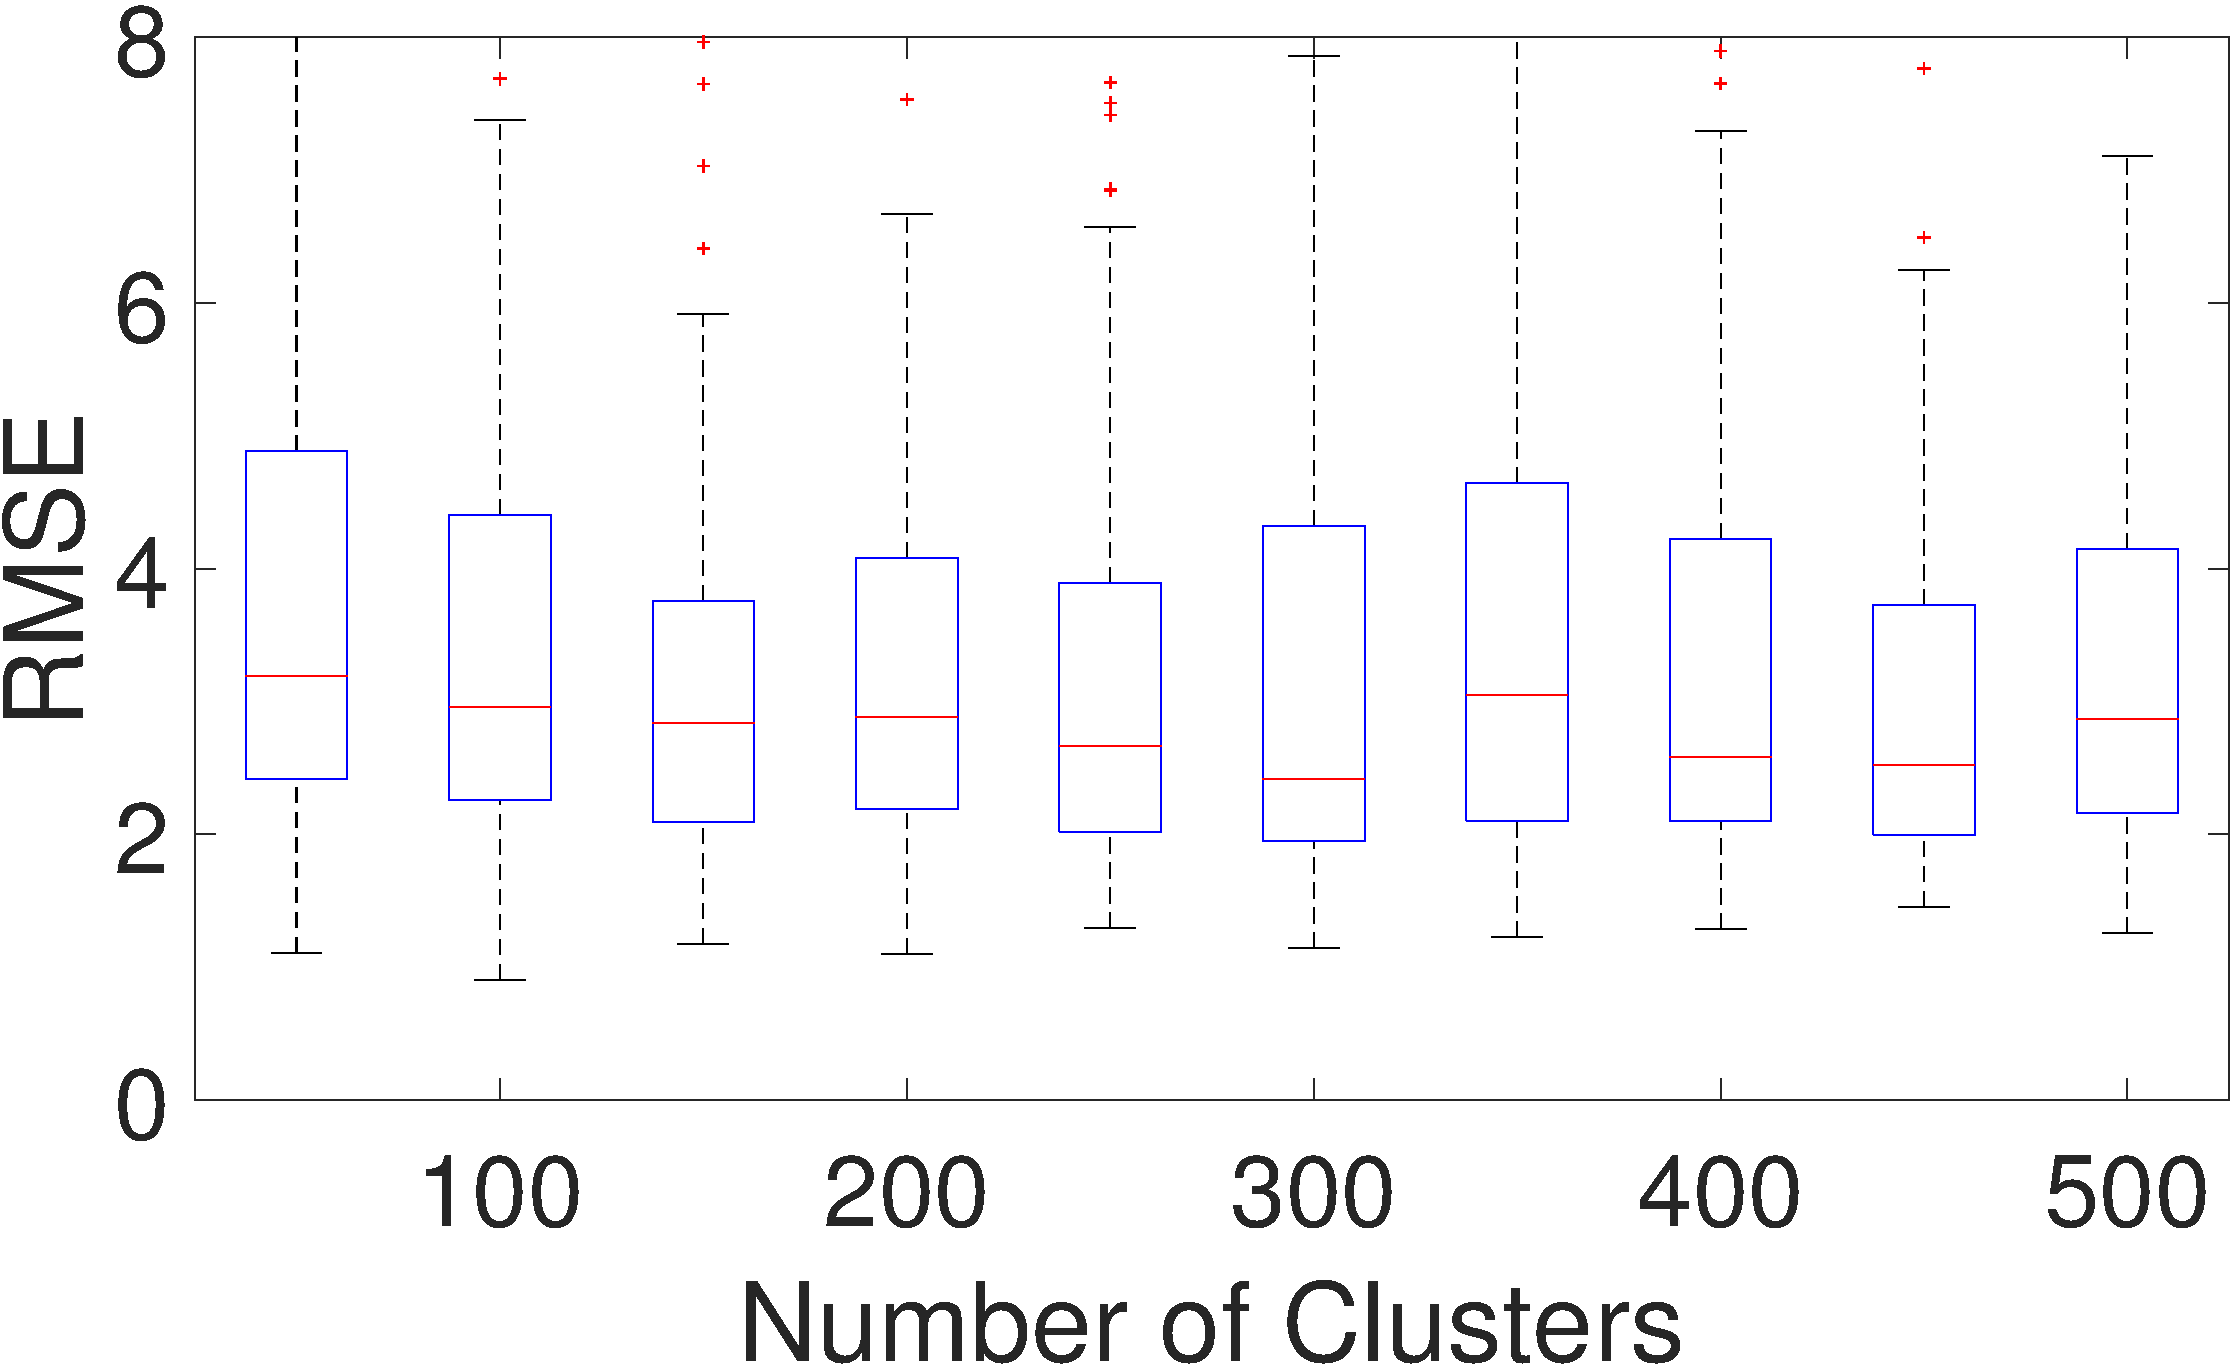
\includegraphics[width=0.3\textwidth]{Figures/RMSE_NbClusters_KNN5}}
\subfigure[$K$=10]{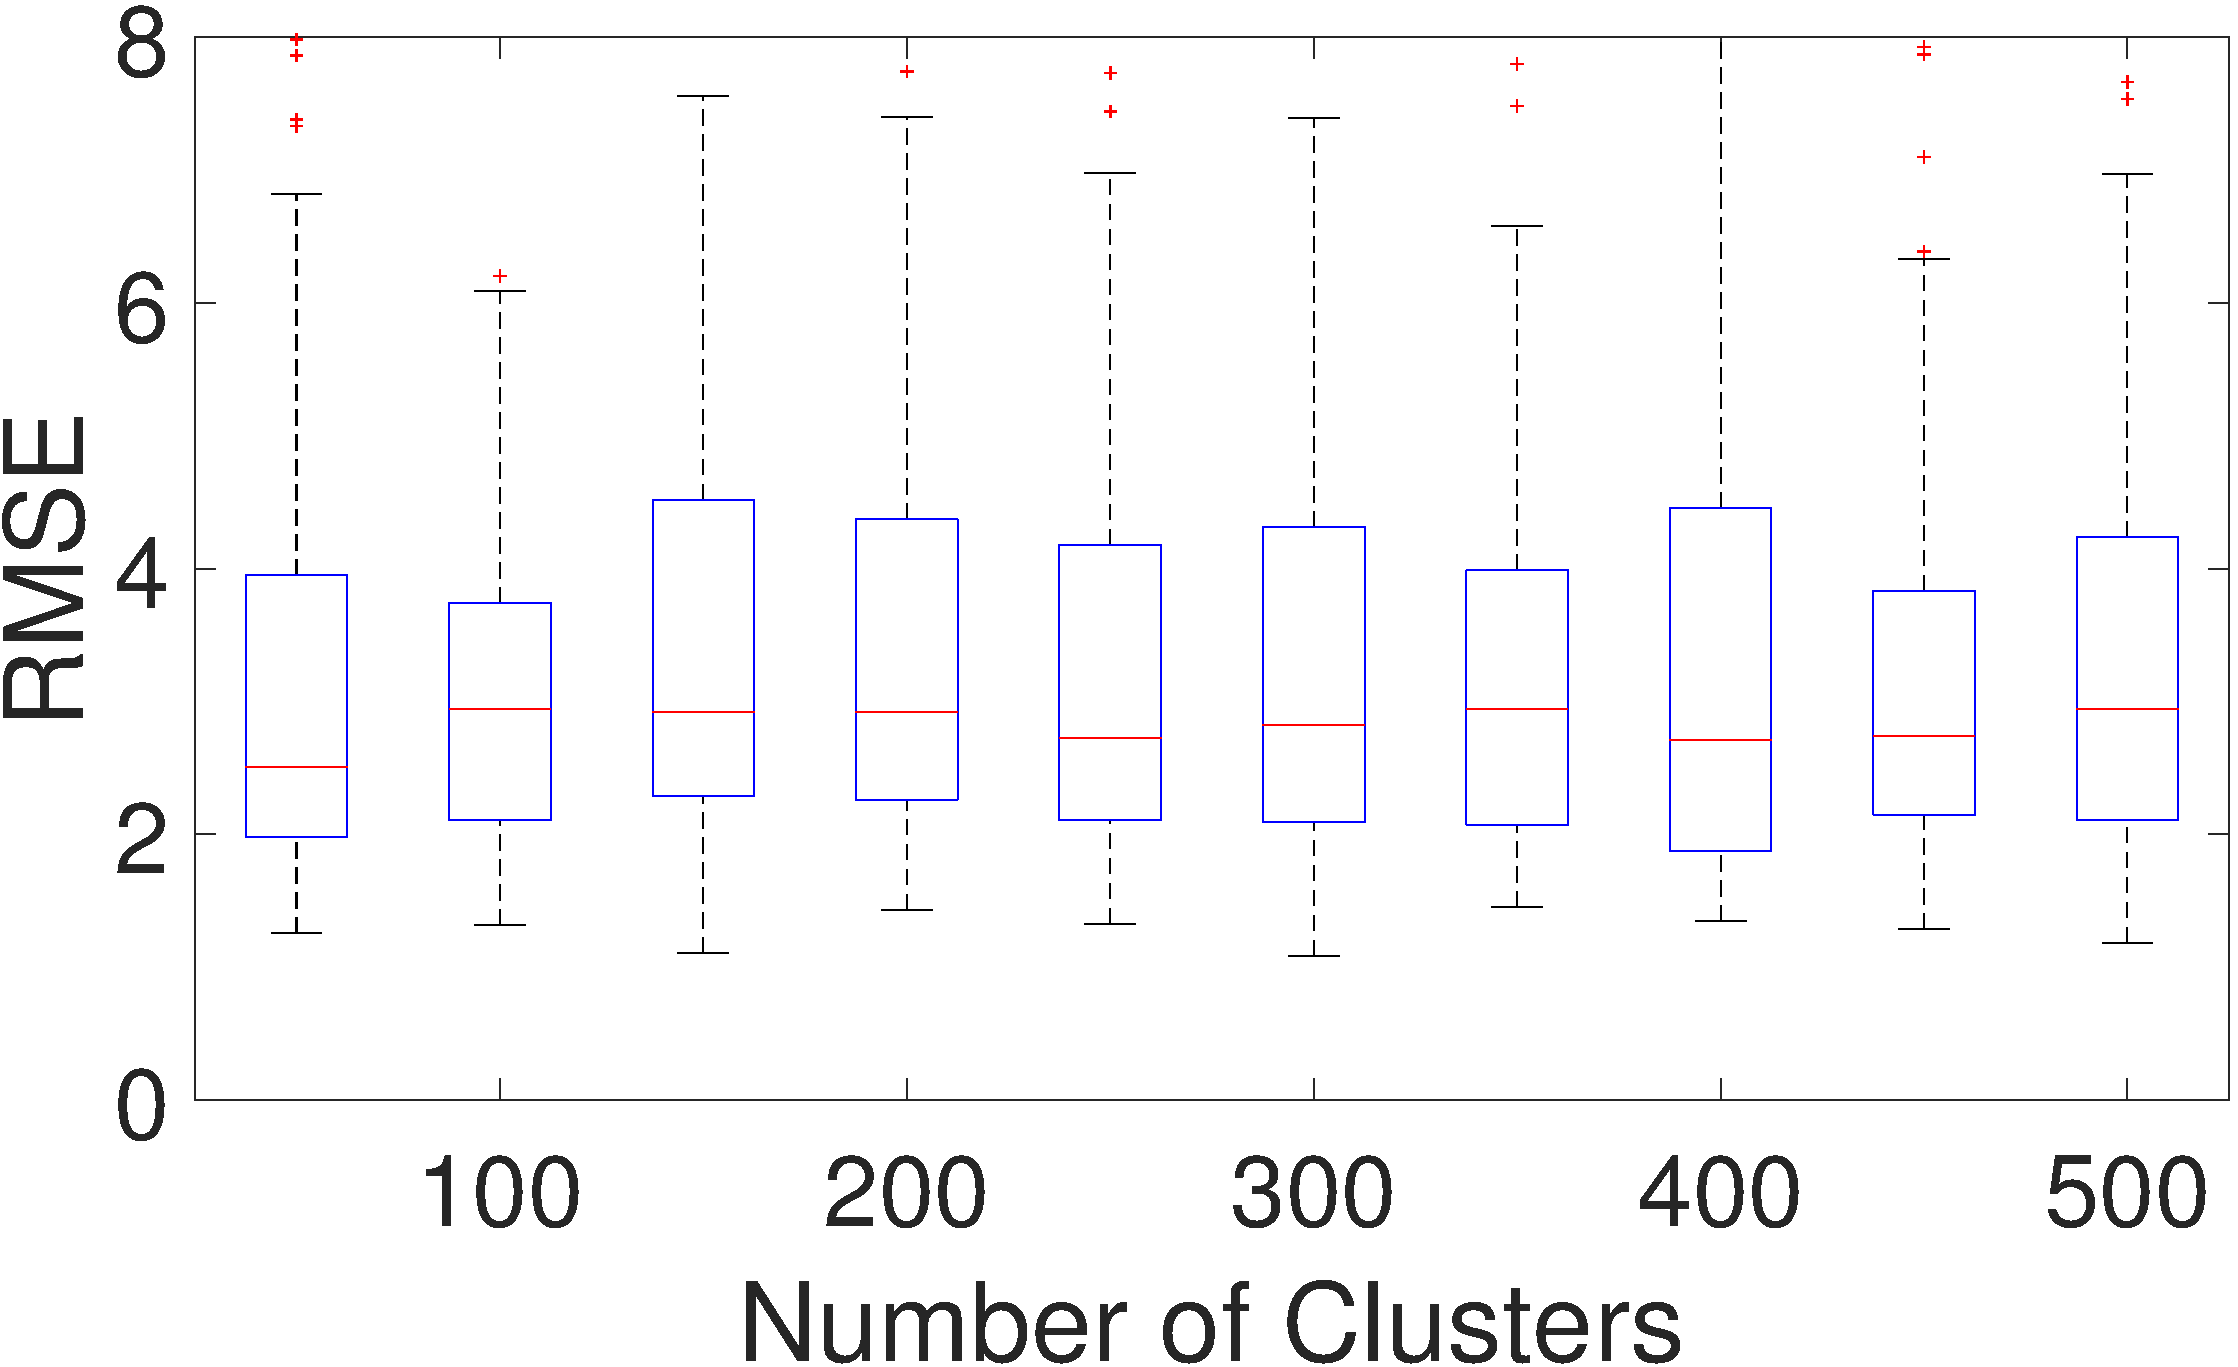
\includegraphics[width=0.3\textwidth]{Figures/RMSE_NbClusters_KNN10}}
\subfigure[$K$=20]{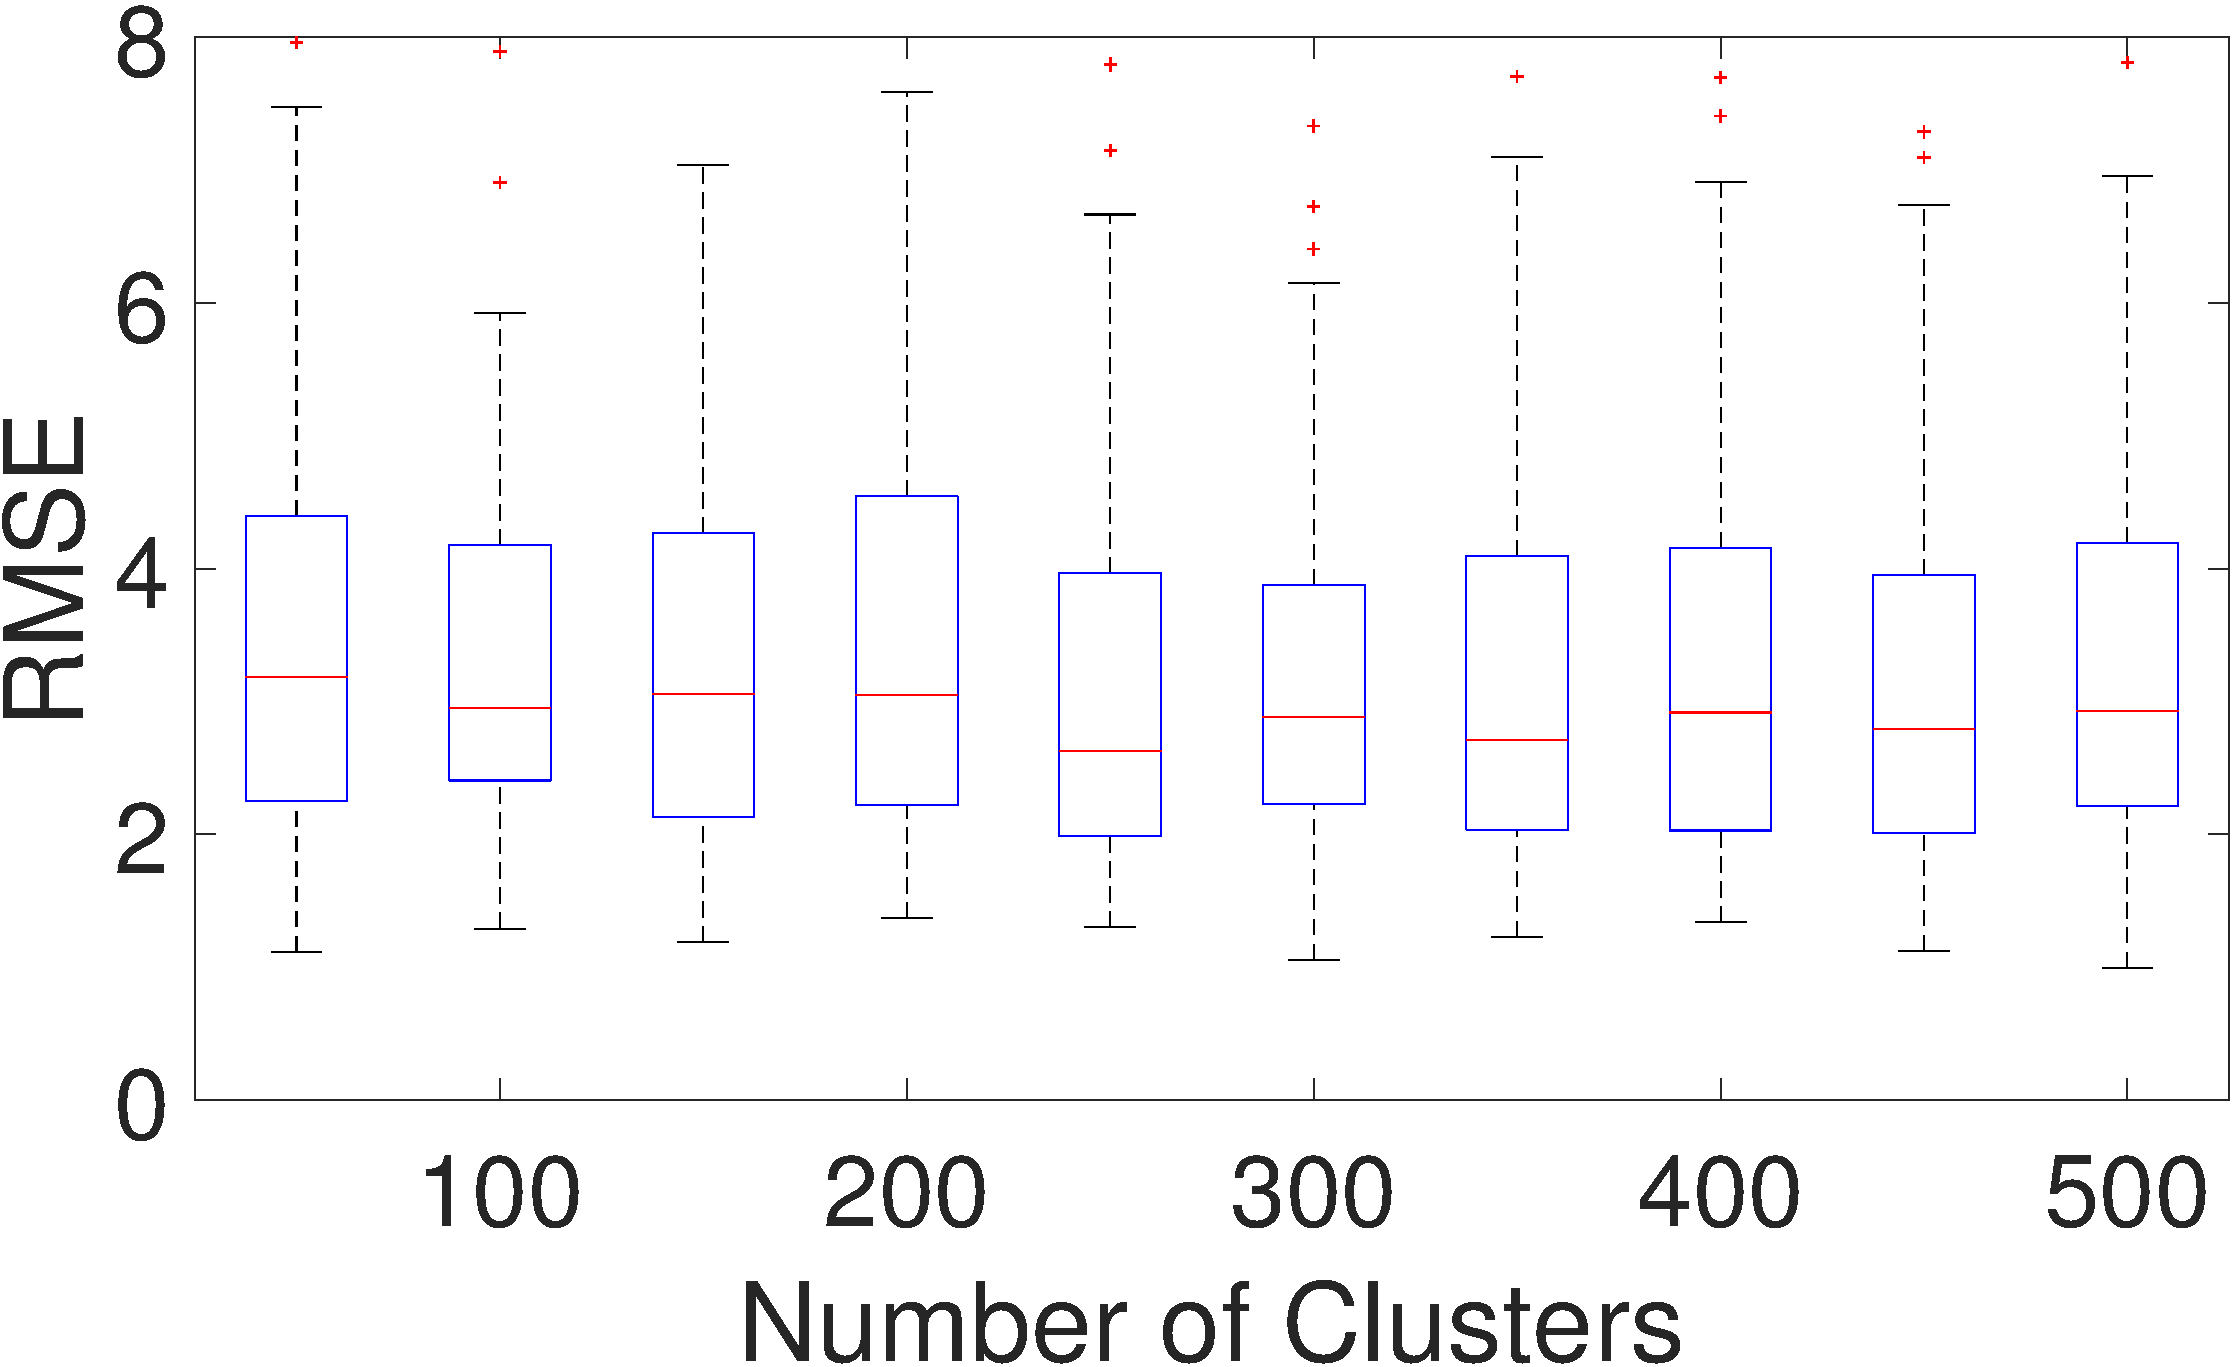
\includegraphics[width=0.3\textwidth]{Figures/RMSE_NbClusters_KNN20}}
\caption{Boxplot of time-averaged RMSE of Clusterpf with respect to the number of eigenvectors over 100 Monte Carlo trials for different values of $K$.}
\label{fig:RMSE_NbClusters}
\end{figure}

\begin{figure}
\centering
\subfigure[$K$=5]{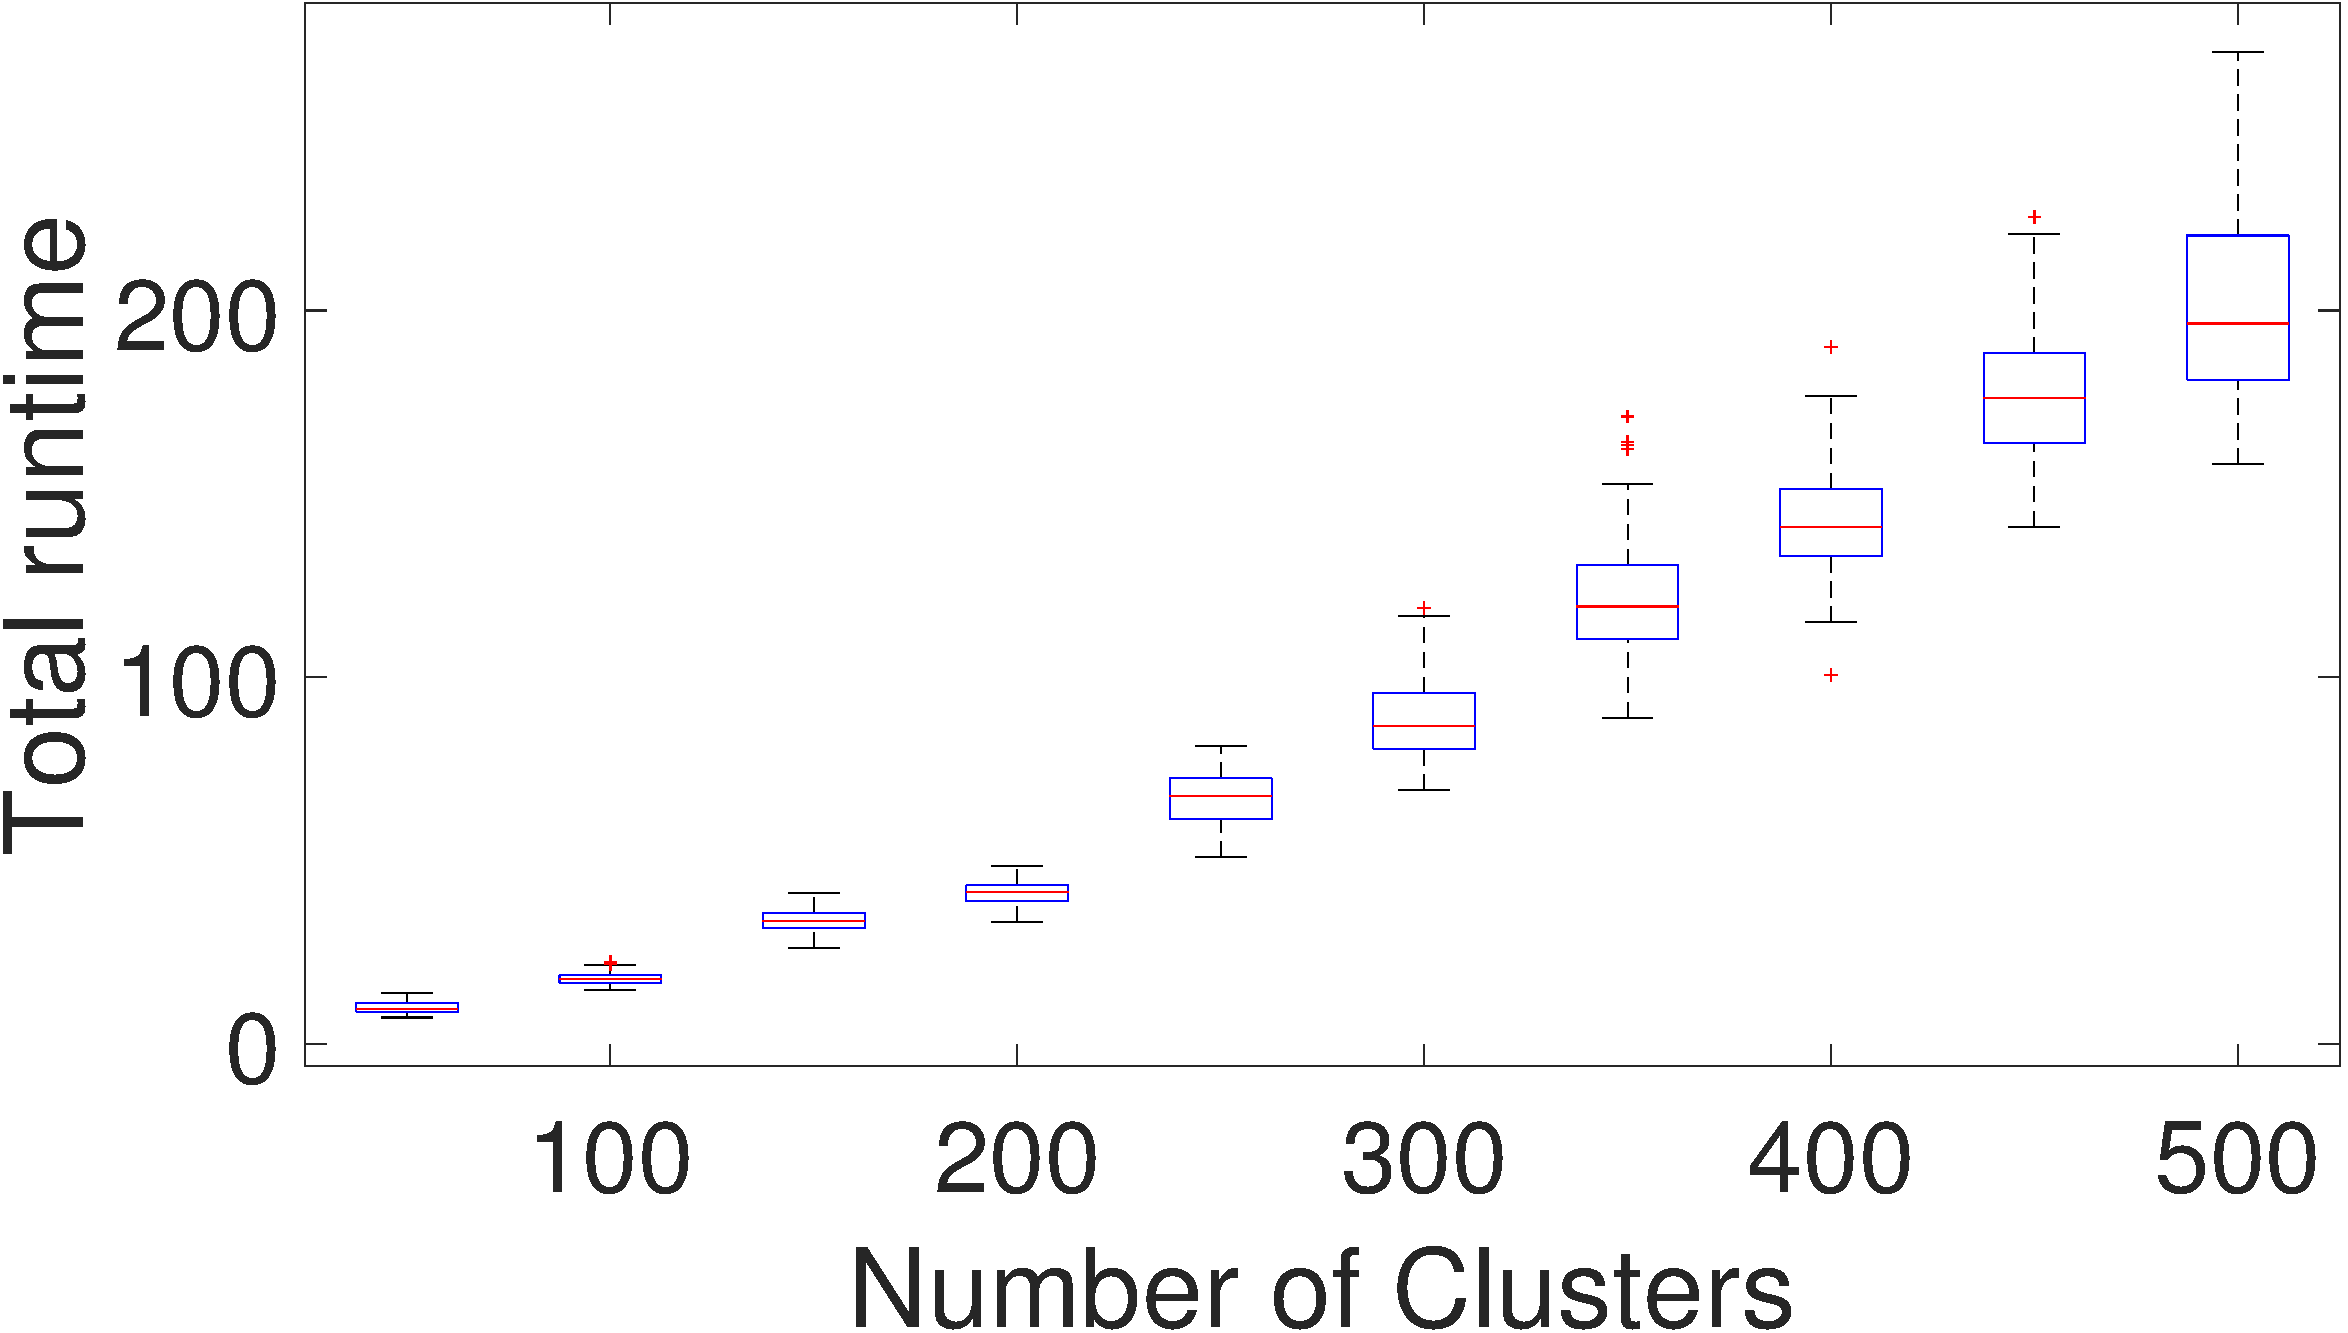
\includegraphics[width=0.3\textwidth]{Figures/runtime_NbClusters_KNN5}}
\subfigure[$K$=10]{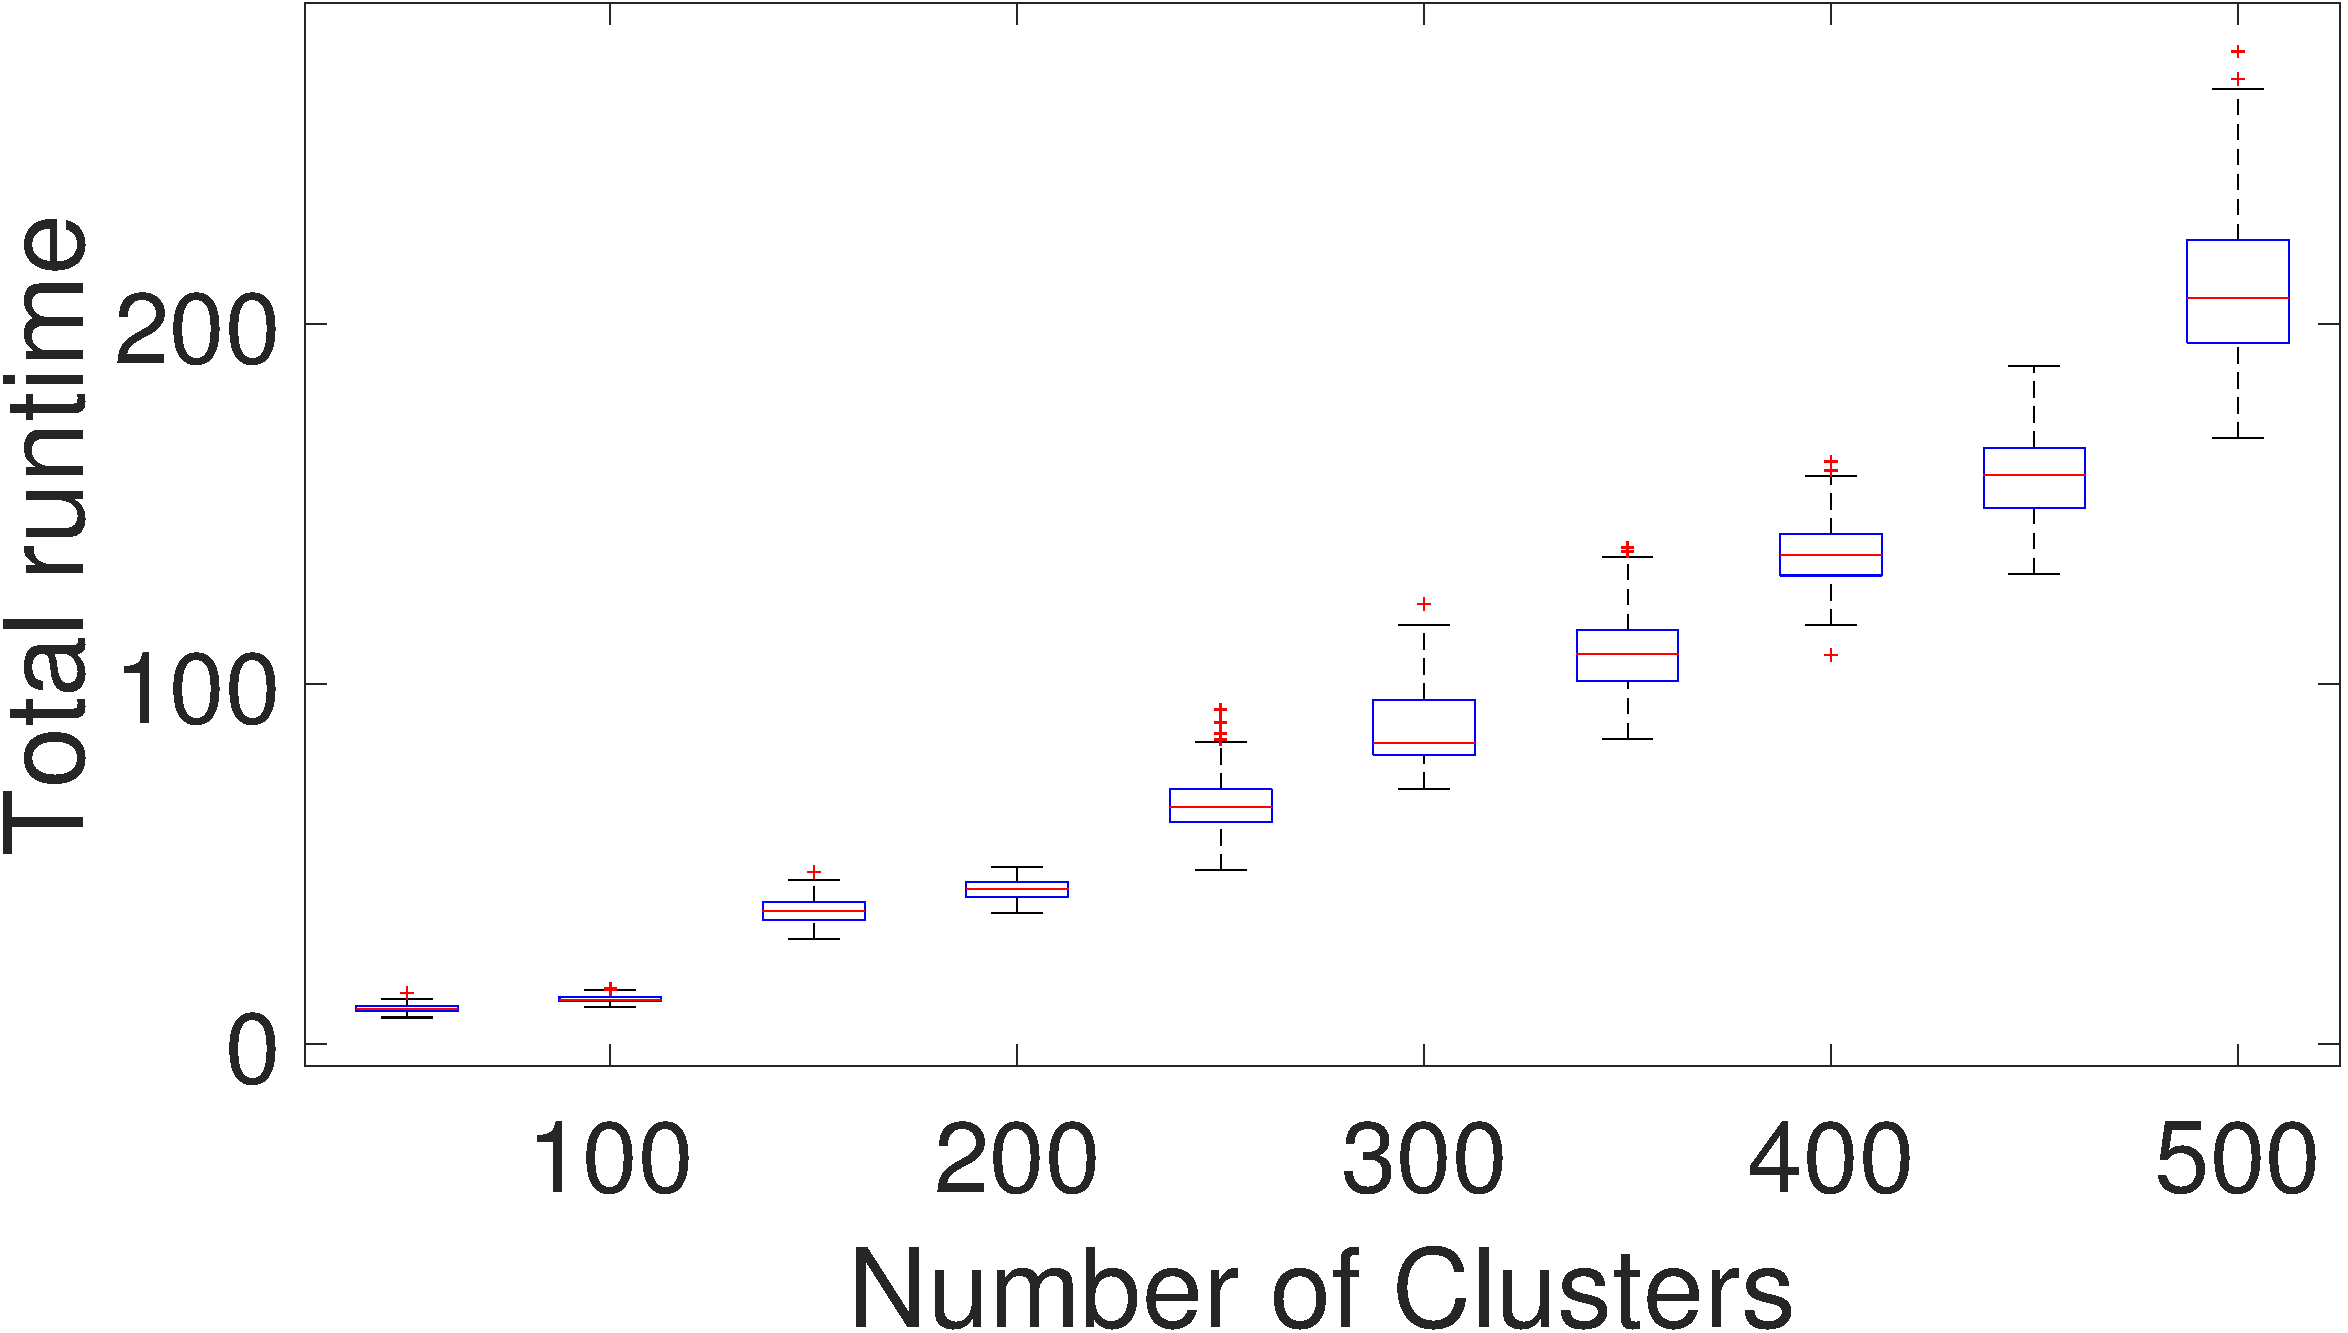
\includegraphics[width=0.3\textwidth]{Figures/runtime_NbClusters_KNN10}}
\subfigure[$K$=20]{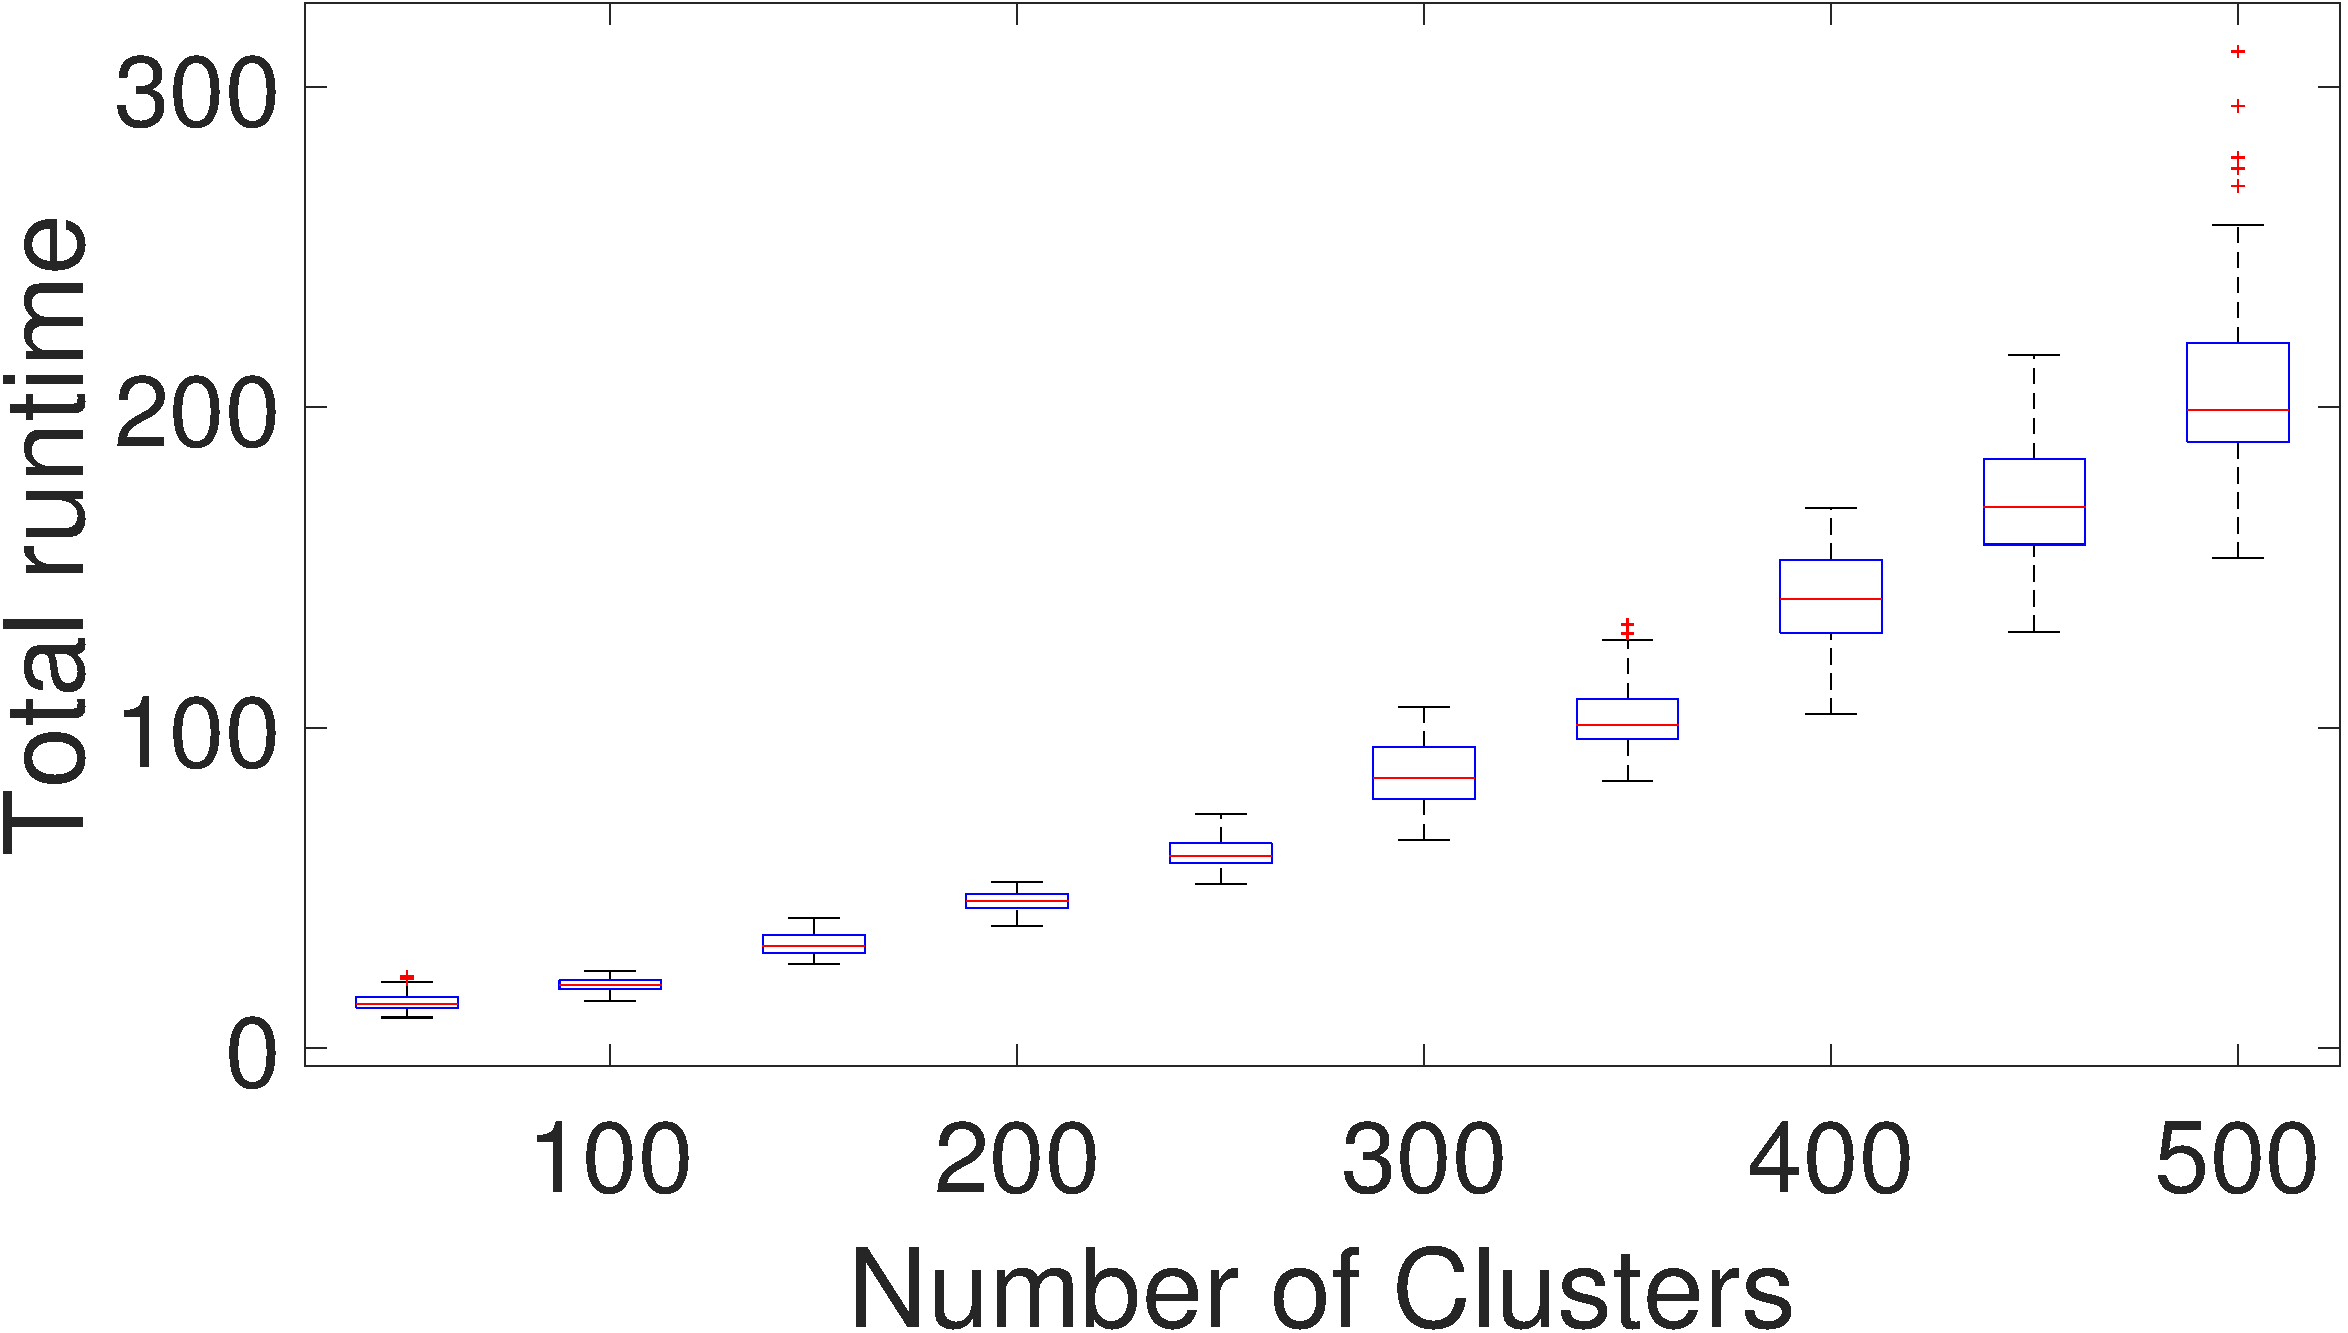
\includegraphics[width=0.3\textwidth]{Figures/runtime_NbClusters_KNN20}}
\caption{Boxplot of total runtime of Clusterpf with respect to the number of eigenvectors over 100 Monte Carlo trials for different values of $K$.}
\label{fig:runtime_NbClusters}
\end{figure}

\subsection{Performance comparison between filters}
To be completed
%Fig.~\ref{fig:MSE} shows the boxplots of mean squared position error with respect to the number of particles. All results are averaged over 100 Monte Carlo trials. At each trial, the trajectory and sensor measurements change. For any trial, all algorithms have the same initial particles and measurements. 

%\begin{figure}
%\centering
%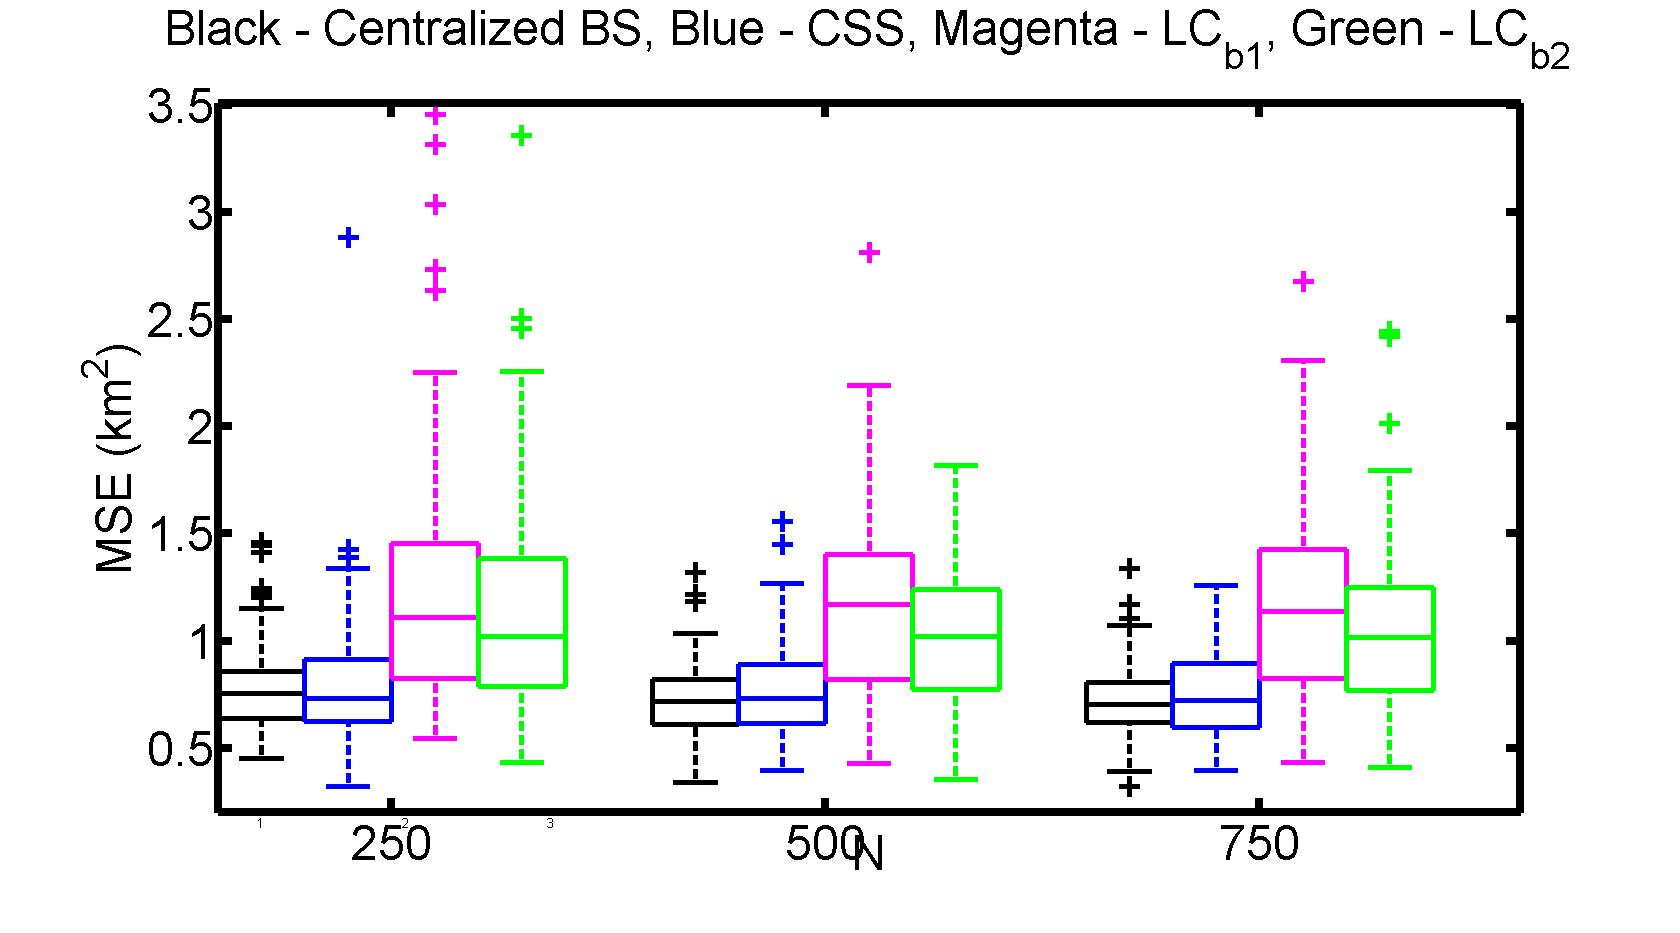
\includegraphics[width=0.75\textwidth]{Figures/MSE}
%\caption{Mean squared position error with respect to number of particles}
%\label{fig:MSE}
%\end{figure}

%The BSPF and CSSPF have similar tracking performance; however the LCPF has consistently the worst performance (i.e., almost double the MSE of the other methods). 

%To understand the poor performance of LCPF, at each time step of BSPF, we compute the particle likelihoods exactly and using likelihood consensus approximation, and then compute the discrepancy between them. Fig.~\ref{} shows the average discrepancy over time. 

\section{Conclusion}
\label{sec:conclusion}
To be completed

\end{document}